%\documentclass[11pt]{report}
%\usepackage{siunitx}
%\usepackage{graphicx}
%\usepackage{multirow}
%\usepackage[table,xcdraw]{xcolor}
%\usepackage{amsmath}
%\usepackage{longtable}
%
%\begin{document}
%\setcounter{chapter}{4}
%\tableofcontents



\newpage
\chapter{Numerical modelling of capacitive-coupled stimulation}
This chapter contains the results of the numerical modelling approaches applied to capacitive-coupled setups to predict the generated electric field. This chapter describes the work presented in the following published works:
\begin{itemize}
\item \small \textit{Meneses, Joao, Sofia R. Fernandes, Nuno Alves, Paula Pascoal-Faria, and Pedro Cavaleiro Miranda. 2021. “Effects of Scaffold Electrical Properties on Electric Field Delivery in Bioreactors.” Conference Proceedings: Annual International Conference of the IEEE Engineering in Medicine and Biology Society. IEEE Engineering in Medicine and Biology Society. Conference 2021 (November): 4147–51.};
\item \small \textit{Meneses, João, Sofia Fernandes, Nuno Alves, Paula Pascoal-Faria, and Pedro Cavaleiro Miranda. 2022. “How to Correctly Estimate the Electric Field in Capacitively Coupled Systems for Tissue Engineering: A Comparative Study.”, Scientific Reports 12 (1): 12522.};
\end{itemize}


\newpage
\section{Introduction}

As defined in Chapter 1, \acs{CCoupled} setups are composed of two electrodes physically separated from the cell culture medium through an electric insulator material, usually an air gap or a petri dish wall. This electric insulator layer obstructs any electron transfer reactions, so the electric signal propagation to the cell culture medium is only possible through a time-varying electric displacement field. This displacement field polarizes the insulator material layers and the cell culture medium trapped between them. In the insulator, the polarization mechanism involves aligning electric dipoles with the applied \acs{EF} (complete absence of free charges). On the other hand, in the culture medium, polarization occurs due to the flow of (free) charged particles, usually ions. The resultant polarization will originate an \acs{EF} in the dielectric medium (insulator layers plus cell culture medium) that opposes the direction of the initially applied \acs{EF} \cite{Ida_undated-cu}. 

Accurate estimates of the \acs{EF} applied by CCoupled setups are essential to compare results from different studies and establish a relation between stimulus characteristics and specific cellular effects. However, this quantity is rarely measured and often estimated with incorrect assumptions of the underlying physics. This chapter includes two works performed on modelling \acs{CCoupled} setups to help understand which factors most affect the generated \acs{EF} delivery for this particular stimulation setup.   

The first work investigated the influence of scaffolds on the \acs{EF} delivered inside a bioreactor \acs{CCoupled} setup, since it constitutes an effect often neglected. Multiple electrical conductive and non-conductive biomaterials have been developed for \acs{BTE} cell culture substrates in a variety of forms (porous scaffolds, films, nanofibers, coatings) \cite{Dong2020}. After cell seeding, this structure is subjected to an electrical stimulation employing, for example, \acs{CCoupled} setups to achieve the desired cell function modulation. The ubiquitous use in the literature of cell support materials in experimental protocols applying electrical stimulation should be addressed in terms of their impact in the \acs{EF} at cellular targets. This impact should then be considered when selecting the scaffold geometry and/or material, in order to ensure no interference or even synergy with the induced \acs{EF}. In this work, we considered the \acs{CCoupled} setup based on Brighton's original work \cite{Brighton1988-vc, Brighton1992-gg} to analyze the impact of a scaffold insertion in the \acs{EF} characteristics. A geometrical model for this setup was created, and a sensitivity analysis was performed using the \acs{FEM}. After validating our model with the experimental measures made by Brighton \textit{et al.} \cite{Brighton1988-vc, Brighton1992-gg} in an empty chamber, an orthogonal scaffold was introduced in the culture medium, and an extensive sensitivity analysis of the delivered \acs{EF} was performed for different values of function of the electrical conductivity and permittivity of the scaffold material and culture medium. Understanding the influence of scaffold geometry and material composition in the delivery of \acs{CCoupled} \acs{EF}s will allow the building of precise, reliable, and replicable stimulation protocols.   

The second work reported in this chapter applies modelling methods to \acs{CCoupled} systems reported in previous literature to corroborate estimates of the \acs{EF} in the culture medium. For this purpose, eight \acs{CCoupled} studies were analyzed as shown in Figure \ref{fig5d1}. The fundamental physics underlying \acs{CCoupled} stimulation were reviewed, and then, three modelling approaches were delineated to estimate the \acs{EF}: two of them based on solving an analog electric circuit model, the first by solving analytically the circuit to find the electric current in the culture medium and the produced \acs{EF}, the second by performing the same steps using LTSpice as a solver, an analog electronic circuit simulator computer software (allowing more complex waveform solutions); the third and last approach was to apply the \acs{FEM} to model the \acs{CCoupled} system geometry and solve it with a golden standard software. A free, open-source tool was developed to perform the models using the first approach and ease future calculation of the \acs{EF} being delivered by \acs{CCoupled} systems in \acs{TE} and \acs{BTE} applications. This \acs{EF} Calculator for \acs{CCoupled} systems is available for download from Zenodo hosting platform \cite{Meneses2022-yk}. An extremely large span of \acs{EF} strengths in the culture medium has been reported for \acs{CCoupled} setups alone, ranging from \num{1.0d-5} \si{\volt\per\meter} \cite{Fitzsimmons1986-ks} to \num{1.7d5} \si{\volt\per\meter} \cite{Rodan1978-yu}. In these studies, different methods were used to estimate the \acs{EF} strength, some of them flawed. Yet, they all describe a positive effect of electrical stimulation on cell culture, and some of them are widely cited. This work aims to determine the validity of the \acs{EF} strength estimated in several \acs{CCoupled} \textit{in vitro} studies by comparing it with the predictions from three different modelling approaches. This work also presents a solid theoretical and practical methodology to estimate the \acs{EF} in \acs{CCoupled} stimulation protocols, thus contributing to enhance reproducibility and help to establish guidelines when \acs{CCoupled} systems are used in \acs{BTE} applications.

\begin{figure}[h]
\makebox[\textwidth][c]{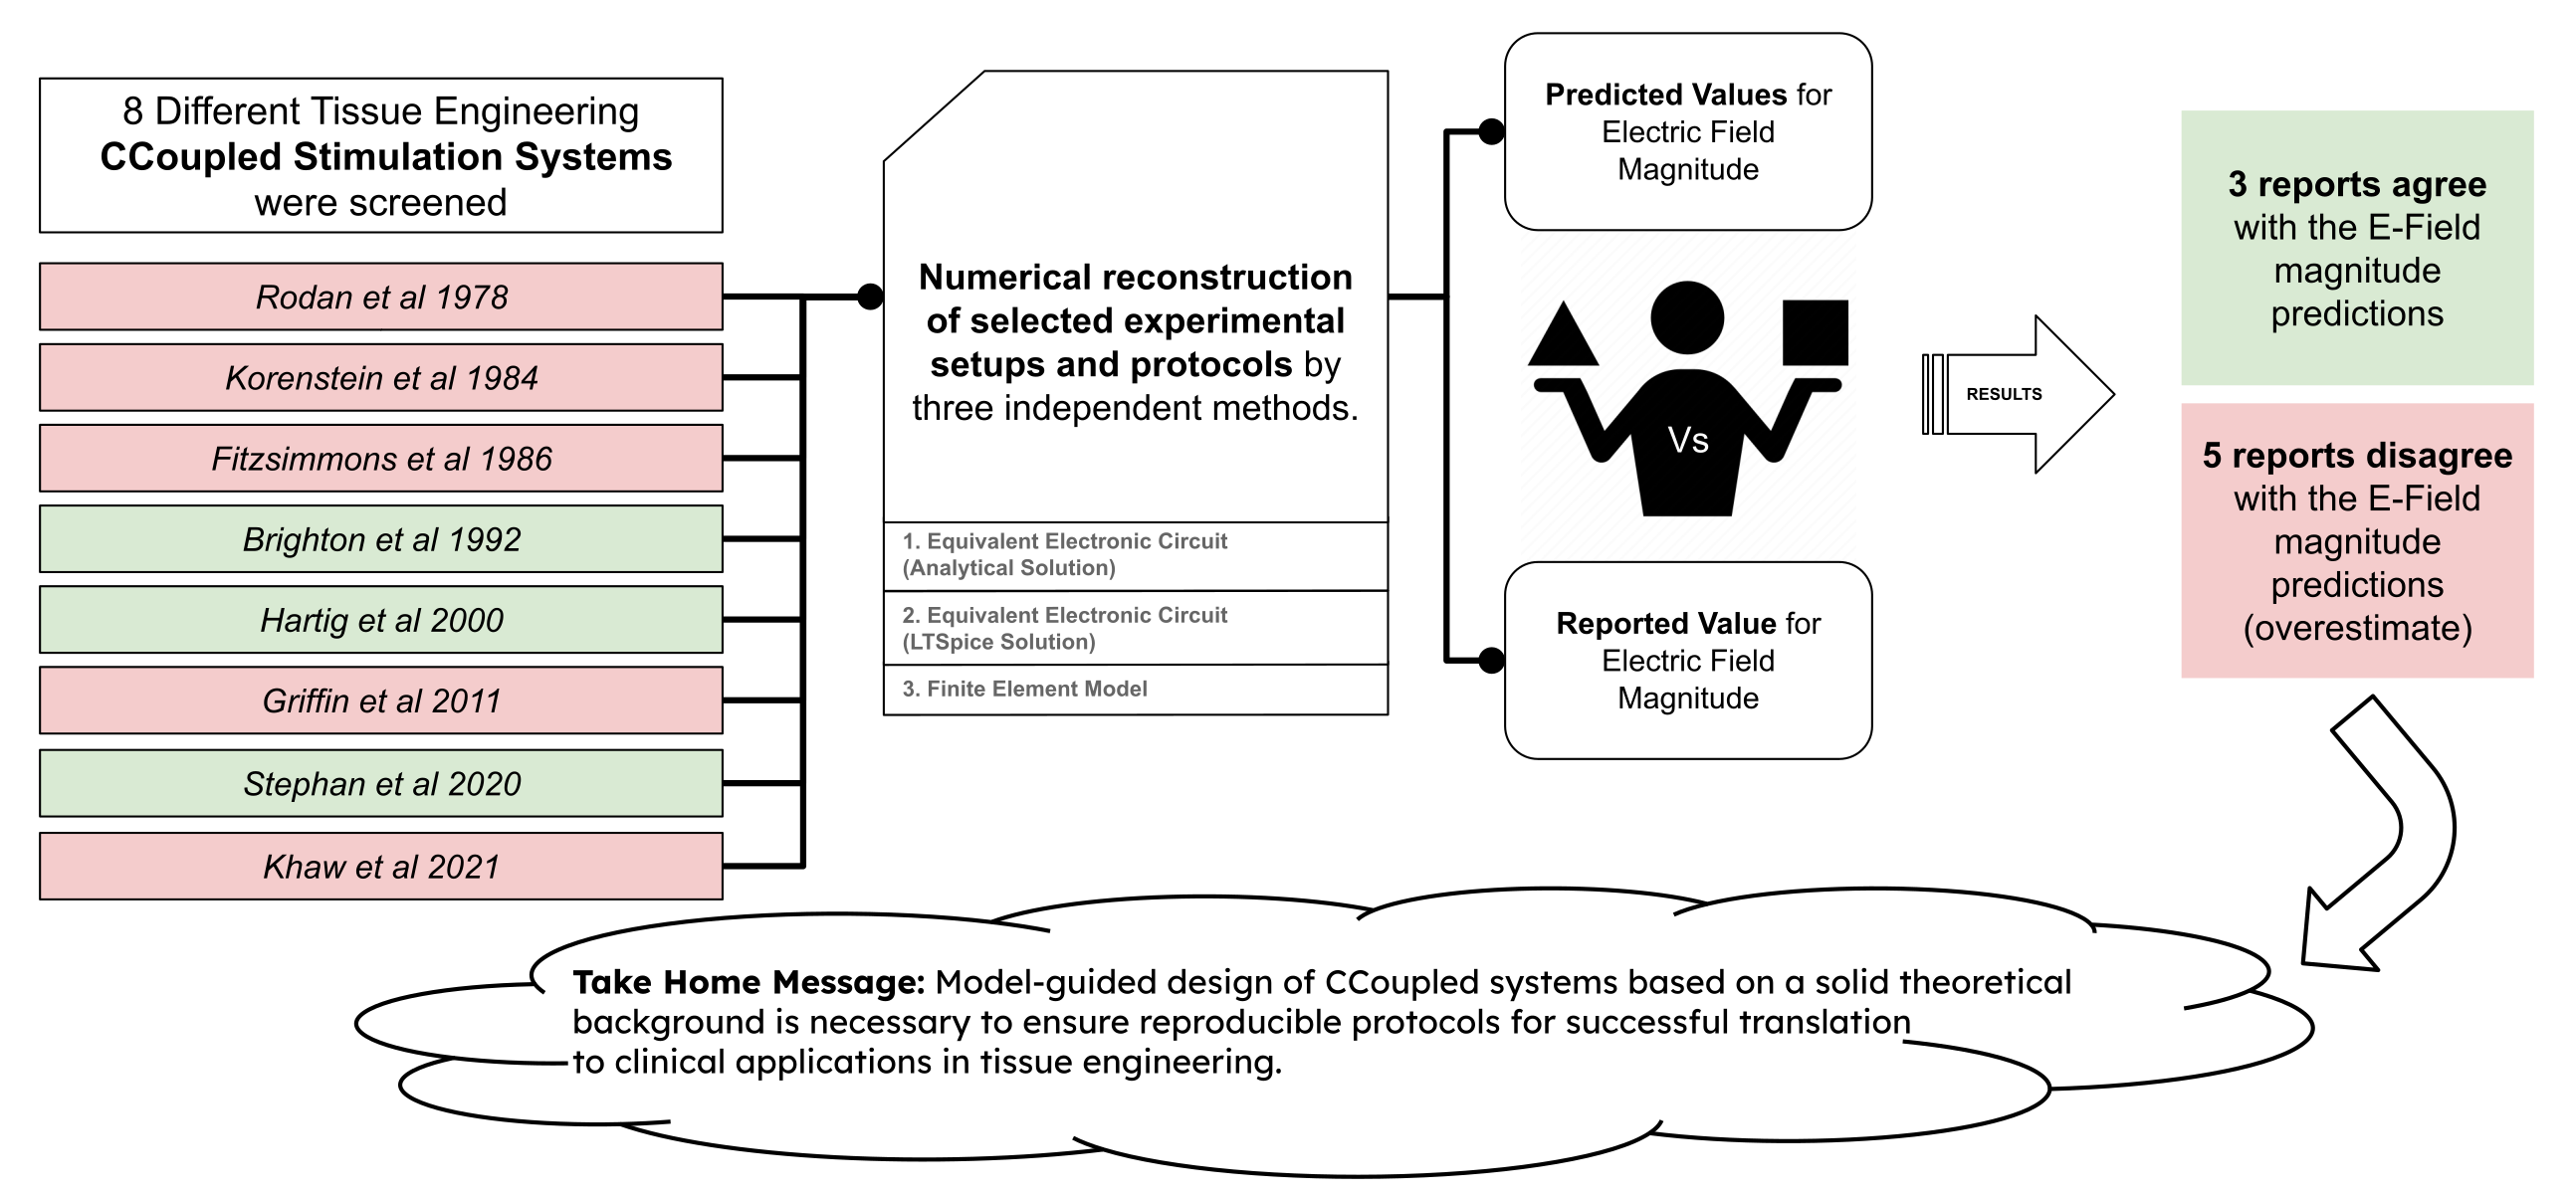
\includegraphics[scale=0.55]{./figures/Figure_5d1.png}}
\caption{Graphical abstract for the work of modelling published CCoupled setups in \acs{BTE}.}
\label{fig5d1}
\end{figure}




\section{Aim}
\begin{itemize}
\item To model the effects of adding scaffold structures into the empty cell culture chamber (containing just culture medium) of an existent \acs{CCoupled} setup;
\item To model the \acs{EF} that is delivered by several reported \acs{CCoupled} setups and protocols, comparing their predictions with the values obtained from the literature;
\end{itemize}




\section{Methods}




\subsection{Scaffold insertion effects}

\textit{Brighton \acs{FEM} Model - Cell Culture Chamber Without Scaffold.} The \acs{3D} model replicating Brighton's experimental setup, as described in \cite{Brighton1988-vc, Brighton1992-gg}, was constructed using SOLIDWORKS software (version 2018, Dassault Systemes SolidWorks Corporation, France). The geometry is composed of 5 co-axial cylindrical domains with a diameter of 33 \si{\milli\meter} (see Figure \ref{fig5d2}A): two stainless steel electrodes, with a thickness of 1 \si{\milli\meter}; two glass coverslips placed between the electrodes and the culture medium, with a thickness of 0.16 \si{\milli\meter}; one cell culture medium chamber that occupies the entire central region, with a thickness of 10 \si{\milli\meter}. The dimensions not specified in Brighton's setup descriptions were estimated based on the drawing from its 1992 manuscript \cite{Brighton1992-gg} and similar commercially available parts. \hfill \break


\begin{figure}
\makebox[\textwidth][c]{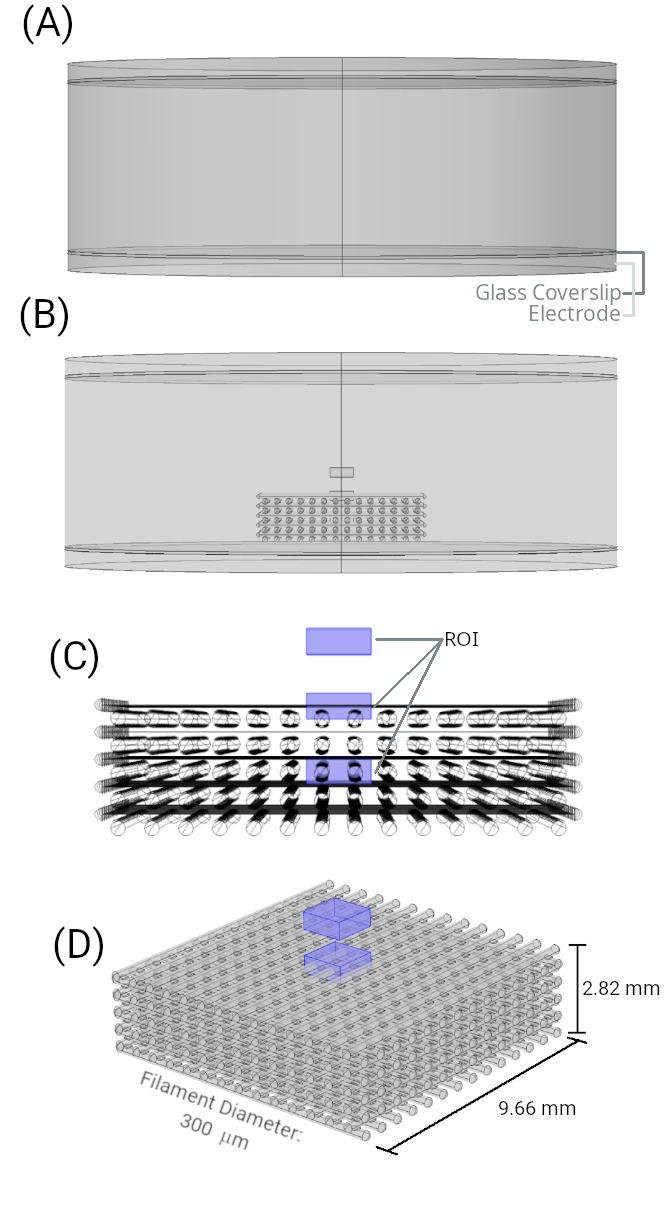
\includegraphics[scale=1.0]{./figures/Figure_5d2.png}}
\caption{Model geometry. (A) \acs{3D} model of Brighton's experimental setup, composed of 5 distinct domains: two electrodes (top and bottom); two glass coverslips (top and bottom); and one culture medium domain (central). (B) A \acs{3D} model with orthogonal scaffold placed at the bottom of the cell culture medium chamber. (C) Three equidistant and equal-sized rectangular prism \acs{ROI}s (tinted blue) represent the scaffold environment's external, interface, and internal regions. (D) Volumetric view of the orthogonal scaffold with overall dimensions and the \acs{ROI}s (tinted blue).}
\label{fig5d2}
\end{figure}


\noindent \textit{Brighton \acs{FEM} Model - Cell Culture Chamber With Scaffold.} To the previously described \acs{3D} model, an orthogonal scaffold was added at the bottom of the cell culture medium chamber (see Figure \ref{fig5d2}B). This scaffold comprises alternating horizontal layers of 300 \si{\micro\meter} filaments, whose centers are 600 \si{\micro\meter} apart. Consecutive layers are rotated by 90\si{\degree}. To avoid meshing and numerical problems associated with point contacts and sharp edges, the tips of each filament were rounded, and an overlap of 20 \si{\micro\meter} was introduced between adjacent horizontal layers, which are then separated by 580 \si{\micro\meter}. For the same reason, the bottom of the scaffold is placed 350 \si{\micro\meter}  above the bottom of the chamber. Three equidistant and equal-sized rectangular prism \acs{ROI}s were added to the 3D model to allow detailed studies in these regions (see Figure \ref{fig5d2}C, \ref{fig5d2}D). \hfill \break

\noindent \textit{Numerical Model Parameters.} \acs{FEM} analysis was conducted with the AC/DC module of COMSOL Multiphysics (version 5.2a, Stockholm, Sweden). The Electric Current (ec) physics interface was selected, considering a frequency-domain study at 60 \si{\kilo\hertz}. A \acs{3D} physics-controlled mesh was also generated in COMSOL for each model (with and without scaffold), considering the finer mesh option. Both models are composed of three common materials: stainless steel for electrodes ($\sigma$: \num{4.032d6} \si{\siemens\per\meter}, $\epsilon_r$: 1.0); cover glass N1 insulating walls ($\sigma$: \num{1.0d-13} \si{\siemens\per\meter}, $\epsilon_r$: 6.85); and cell culture medium. The model with scaffold also contains the scaffold material, the properties of which were varied in a parametric sweep study together with the culture medium properties (Table \ref{table_sensitivity}). Following Brighton's work \cite{Brighton1988-vc, Brighton1992-gg}, an electric potential boundary condition of 44.81 \si{\volt} was added to the top surface of the top electrode, and a ground boundary condition was added to the bottom surface of the bottom electrode. COMSOL \acs{BiCGStab} stationary iterative solver was used to run this parametric sweep study, due to its ability to handle a wide range of matrices (memory efficiency), often converging faster than other iterative solvers. \hfill \break



\begin{table}
\caption{Sensitivity Analysis Study Parameters. Selected parameters match common scaffold materials and culture medium properties.}
\bigskip
\scriptsize
\centering
\begin{tabularx}{350px}{l l l} \toprule[0.15em]
& \textbf{Culture Medium}  & \textbf{Scaffold}  \\ \cmidrule(l){1-3}
\textbf{Electrical Conductivity} $\sigma_{cm}$ (\si{\siemens\per\meter}) & \textit{1.1, 1.5, 1.9} & \textit{\num{1.0d-14}, 0.001, 0.005, 0.01, 0.05,} \\
& & \textit{0.1, 0.5, 1.1, 1.3, 1.5, 1.7, 1.9, 10, 50,} \\
& & \textit{100, 150, 300, 500, 1000, \num{7.5d5}} \\
\textbf{Relative Permittivity} $\epsilon_{cm}$ (dimensionless) & \textit{50, 80.1, 90} & \textit{1, 2.2, 80.1} \\ \bottomrule[0.15em]
\end{tabularx}
\label{table_sensitivity}
\end{table}


\noindent \textit{Sensitivity and Spatial Distribution Analysis.} Sensitivity analysis was performed employing a one-at-a-time variation method, applied to the results obtained from the COMSOL parametric sweep study. This parametric sweep study generated 540 different solutions, one for each combination of the input parameters described in Table \ref{table_sensitivity}, with electrical conductivities and permittivities values obtained from \cite{Gavish2016-av, Bennett2019-js, Mazzoleni1986-wp}. \acs{EF} data were then exported from COMSOL Multiphysics software to text file format for further postprocessing in custom-made Python scripts (using Pandas, Matplotlib, and SALib libraries). These Python scripts were used to generate the plots and histograms for sensitivity and spatial distribution analysis. Sensitivity analysis was performed by the method of Delta Moment-Independent Measure, implemented in the python SALib library, according to the original works of Borgonovo \textit{et al.} and Plischke \textit{et al.} \cite{Borgonovo2007-tj, Plischke2013-ok}. Sensitivity and spatial distribution analysis were independently performed for each \acs{ROI} (external, interface, and internal), where only the culture medium nodes data were considered. Spatial distribution analysis was performed on three authentic scaffold materials from the \acs{TE} field (Thermoplastic \cite{Hegde2015-nd}, Hydrogel \cite{Distler2020-gi}, Metalic \cite{MetalInfo}), and also on a control scaffold with the same material electrical properties of the cell culture medium (no effect of scaffold presence is expected under this condition).


\subsection{Modelling \acs{CCoupled} reported setups}


\noindent \textit{Electric Circuit Model of \acs{CCoupled} Experimental Setups.} The geometry of experimental setups for \acs{CCoupled} electrical stimulation of cells can often be modeled as shown in the previous section by using a cylindrical layered geometry, with two circular metallic plates separated from the culture medium by electrically insulating layers, typically plastic, glass, or air, as shown schematically in Figure \ref{fig5d3}a. Note that all layers have the same diameter in this model. Given the setup's geometry, the electric charge flows parallel to the cylinder's axis.  In general, each layer can be described in terms of a resistor and a capacitor in parallel (Figure \ref{fig5d3}b) since both paths are available for the flow of charge.


\begin{figure}
\makebox[\textwidth][c]{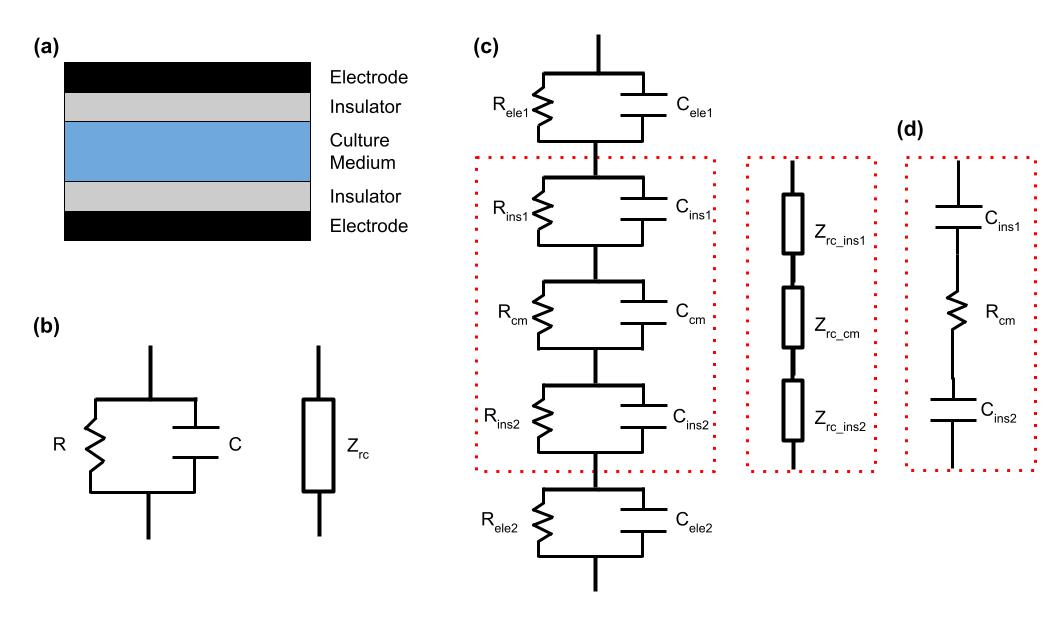
\includegraphics[scale=1.5]{./figures/Figure_5d3.png}}
\caption{(a) Layered cylindrical model of a typical \acs{CCoupled} experimental setup; (b) Resistor-capacitor (RC) model and impedance circuit model for an individual layer; (c) RC and impedance circuit models for the five layers; (d) The complete circuit can be reduced to its three most relevant components without significant loss of accuracy. Abbreviations: ele-electrode, ins-insulator, cm-culture medium, r-resistor, c-capacitor, z-impedance.}
\label{fig5d3}
\end{figure}

In this geometry, the \acs{EF} within each layer is uniform so the resistance, $R_i$, and capacitance, $C_i$, of the $i^{th}$ layer are given by the familiar formulae,

\begin{equation}
\label{eq2}
R_i = \rho_i \frac{l_i}{A}
\end{equation}

\begin{equation}
\label{eq3}
C_i = \frac{\epsilon_{0} \epsilon_{r_i} A}{l_i}
\end{equation}

\noindent where $\rho_i$ is the resistivity of the material, $\epsilon_{r_i}$ its relative permittivity and $\epsilon_{0}$ the permittivity of vacuum, $A$ is the cross-sectional area of the cylinder and $l_i$ the thickness of the layer. The relation between the current, $I$, which is the same in all layers due to charge conservation, and the voltage drop in each layer, $V$, is given by Ohm’s law

\begin{equation}
\label{eqOhms}
V_i = Z_i I
\end{equation}

\noindent where $Z_i$ is the impedance of the $i^{th}$ layer. Note that this is the impedance of the resistor, $Z_r$, and of the capacitor, $Z_c$, in parallel, i.e.,

\begin{equation}
\label{eqLayerimpedance}
\frac{1}{Z_{i}} = \frac{1}{Z_{r_i}} + \frac{1}{Z_{c_i}}
\end{equation}

The impedances of the resistor and capacitor are defined by:

\begin{equation}
\label{eqRimpedance}
Z_{r_i} = R_i
\end{equation}

\begin{equation}
\label{eqCimpedance}
Z_{c_i} = j X_{c_i} = -\frac{j}{\omega C_i}
\end{equation}

\noindent where $X_{c_i}$ is the capacitive reactance, $\omega$ is the angular frequency of the applied sinusoidal signal, and $j$ is the imaginary unit. Thus

\begin{equation}
\label{eqLayerimpedance2}
\frac{1}{Z_{i}} = \frac{1}{R_i} + j \omega C_i
\end{equation}

\noindent or

\begin{equation}
\label{eqLayerimpedance22}
Z_{i} = \frac{R_i (1 - j \omega C_i R_i)}{1 + \omega^{2} C_i^{2} R_i^{2}}
\end{equation}

\noindent Note that impedances are complex numbers and that the impedance of a capacitor is frequency dependent, it decreases with increasing frequency. 

The whole setup can be viewed as a series of five parallel RC circuits, one for each layer (Figure \ref{fig5d3}c) \cite{Wiesmann2001-uh}. The total impedance of the five layers in series is the sum of the individual (complex) impedances,

\begin{equation}
\label{eqTotalimpedance}
Z_{total} = \sum_{i} Z_i.
\end{equation}

\noindent The ratio between the applied voltage, $V$, and the current, $I$, through the setup is given by the total impedance, $Z_{total}$, of the setup, i.e.

\begin{equation}
\label{eqOhms2}
V = Z_{total} I.
\end{equation}

The voltage drop across a single layer, $V_i$, can, therefore, be obtained as a fraction of the applied voltage

\begin{equation}
\label{eqOhms3}
V_i = Z_{i} I = \frac{Z_i}{Z_{total}} V.
\end{equation}

\noindent Then, the magnitude of the \acs{EF} in a layer is given by

\begin{equation}
\label{eqOhms4}
\lvert E_i \rvert = \frac{\lvert V_i \rvert}{l_i}
\end{equation}

\noindent where $l_i$ is the thickness of the $i^{th}$ layer.

The purpose of this section was to show that for simple geometries like the one considered here it is possible to predict the \acs{EF} in the culture medium, provided that the physical parameters of the setup are known, namely the dimensions $A_i, l_i$ and electrical properties $\rho_i, \epsilon_{r_i}$, and that the applied voltage has a sinusoidal waveform, which is characterized by a single frequency. In fact, the \acs{EF} in the various layers is independent of the (constant) cross-sectional area $A$ because the total impedance of every layer is inversely proportional to $A$ and the \acs{EF} is proportional to a ratio of impedances. 

The model shown in Figure \ref{fig5d3}c is also useful to understand some general features of \acs{CCoupled} setups. It turns out that, in any one layer, the impedance of either the resistive or the capacitive arm is much larger than that of the other arm. For the insulating layers $ Z_{c_i} \ll Z_{r_i} $, whereas for the conductive layers $ Z_{r_i} \ll Z_{c_i} $ (see Table \ref{table_electro} in Results section). In these cases, the equation for the impedance of the $i^{th}$ layer (eq. \ref{eqLayerimpedance}) becomes $Z_i = Z_c$ or $Z_i = Z_r$, respectively. In other words, charge flows almost exclusively through the capacitor in insulating layers, whereas in conductive layers, charge flows almost exclusively through the resistor. In addition, the impedance of the electrodes is very low due to the high conductivity of metals, so the voltage drop across them can be neglected. As a result of these considerations, the circuit in Fig. \ref{fig5d3}c can be represented, to a very good approximation, by a capacitor, a resistance, and a second capacitor in series, as in Fig. \ref{fig5d3}d and in the work of Fitzsimmons \textit{et al.}, Figure 2 \cite{Fitzsimmons1986-ks}. The capacitors represent the insulating layers; whereas the resistor is the culture medium.

In setups commonly used in \acs{TE} the impedance of the culture medium, $Z_r$, is much lower than that of insulating layers, $Z_c , i.e., Z_r \ll Z_c \simeq Z_{total}$. Consequently, the voltage drop across the culture medium is only a tiny fraction of the applied voltage (see eq. \ref{eqOhms3}), and the \acs{EF} in the culture medium is weak. This \acs{EF} can be increased by reducing the impedance of the insulating layers, and hence the total impedance, either by decreasing the thickness of the insulating layers or by working at higher frequencies. It also follows from the equations presented above that, for a fixed capacitive impedance, the \acs{EF} in the culture medium is practically independent of its height (reported as ``thickness" in the tables ahead), provided that $Z_r \ll Z_c$. This is because the impedance of the culture medium is proportional to the thickness of the layer, to a very good approximation (eq. \ref{eq2}), and the \acs{EF} is proportional to the impedance (eq. \ref{eqOhms3}) and inversely proportional to the thickness of the layer (eq. \ref{eqOhms4}).

Another important consequence of the low relative impedance of culture medium ($Z_r \ll Z_c \simeq Z_{total}$) is that the total impedance of the circuit is approximately equal to the impedance of the insulating layers. As a result, the circuit responds almost as a capacitor. For a capacitor with capacitance $C$, the relation between current and voltage is given by 

\begin{equation}
\label{eqRelation}
I = C \frac{\partial V}{\partial t},
\end{equation}

\noindent which is obtained by differentiating $Q = CV$ with respect to time, where $Q$ is the charge stored on the capacitor. The \acs{EF} anywhere in the setup is proportional to the current $I$, so its magnitude is determined primarily by the rate of change of the applied voltage. For a sinusoidal applied voltage, the \acs{EF} in the culture medium will also be sinusoidal with a phase lead of approximately 90\si{\degree} and a magnitude that is proportional to the product of the frequency of the sine wave and of its amplitude (Fig. \ref{fig5d4}a, b). In the case of a trapezoidal pulse, the \acs{EF} will be non-zero only during the risetime and falltime of the pulse and is zero during the plateau. For a linear ramp, the \acs{EF} will be proportional to the wave's amplitude divided by the rise or fall time. Note that the rising and falling edges of the trapezoidal pulse will produce \acs{EF} with opposite directions (Fig. \ref{fig5d4}c, d). More detailed information about the theory of \acs{AC} circuits may be found in Physics or Electrical Engineering textbooks, e.g., \cite[Subchapters 7.2-7.4]{Grant1990}. \hfill \break


\begin{figure}
\makebox[\textwidth][c]{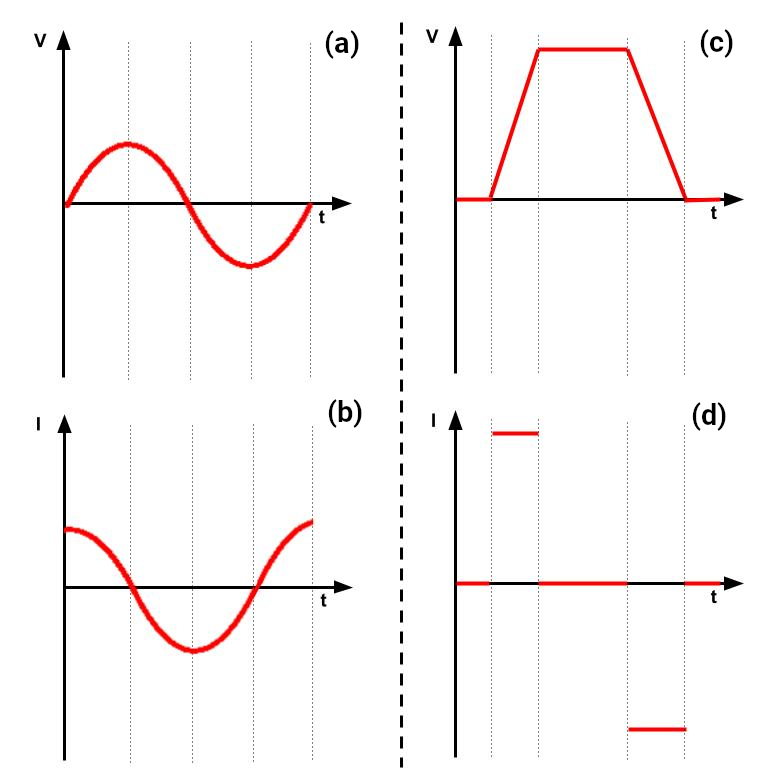
\includegraphics[scale=1.0]{./figures/Figure_5d4.png}}
\caption{Voltage/current waveforms for a purely capacitive circuit. For an input sinewave voltage (a), the resulting current waveform is given by (b). For an input trapezoidal voltage (c), the resulting current waveform in the circuit is (d).}
\label{fig5d4}
\end{figure}


\noindent \textit{Numerical Approaches for Calculating the Electric Field - Analytical approach.} The electrical circuit model described in the previous section can be used to calculate the \acs{EF} in the culture medium for a cylindrical geometry and a sinusoidal applied voltage. The described equations can be easily implemented in Excel, Matlab, or Python, for example. When the waveform is not sinusoidal, an estimate of the maximum \acs{EF} strength can be obtained by considering a frequency such that the maximum rates of change with time of the actual voltage waveform and a sinusoidal waveform of equal amplitude match. For example, for a linear ramp of amplitude $A$ and risetime $\tau$, consider a sinusoidal voltage of amplitude $A$ and frequency $f$. Then, equaling the maximum rates of change of these two waveforms gives the matching frequency:

\begin{equation}
\label{eqFrequency}
\frac{A}{\tau} = 2 \pi f A \quad or \quad f = \frac{1}{2 \pi \tau}
\end{equation}

The proposed analytical approach will yield estimates of the \acs{EF} of the right order of magnitude even when the geometry is non-cylindrical. However, appropriate care must be taken to choose equivalent dimensions for the cylindrical model. Specifically, the thickness of the insulating layers in the cylindrical model should be the same as in the original setup. \hfill \break


\begin{figure}
\makebox[\textwidth][c]{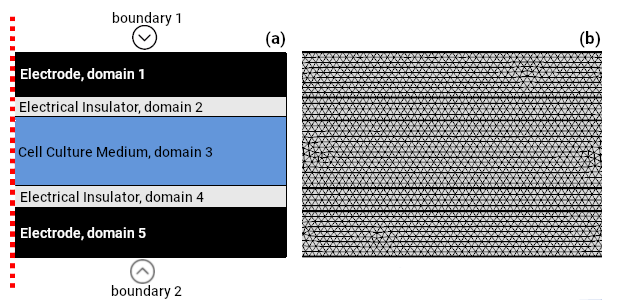
\includegraphics[scale=2.0]{./figures/Figure_5d5.png}}
\caption{Axisymmetric representation of a typical \acs{CCoupled} electric stimulation setup. (a) Domain identification of each layer and electrical boundary conditions applied at the electrodes for \acs{FEM} analysis; (b) Example of a physics-controlled mesh obtained in COMSOL using the extra fine option.}
\label{fig5d5}
\end{figure}

\noindent \textit{Numerical Approaches for Calculating the Electric Field - Circuit simulator approach.} As an alternative to the analytical approach, it is possible to use software packages for the simulation of analog circuits to view the temporal variation of the current or of the voltage drop in the culture medium and to estimate the \acs{EF} strength in the region of interest. We used the freely distributed program LTspice (LTspice LVII, Analog Devices, USA) to draw a circuit like the one illustrated in Fig.\ref{fig5d3}c considering only the 3 central sections since the impedance of the electrodes is negligible. The voltage waveform was specified as a sinusoidal waveform using the SINE option, as a trapezoidal pulse using the PULSE option, or as an arbitrary waveform using the PWL (piece-wise linear) option. After running the simulation, an LTspice probe tool was used to obtain the current through the resistive branch of the culture medium, from which the voltage drop and hence the \acs{EF} were calculated. Note that if using a circuit like the one illustrated in Fig.\ref{fig5d3}d for these simulations, the resistive and capacitive impedances of the various layers were calculated based on a single, matching frequency obtained as outlined in equation \ref{eqFrequency}. The two approaches should therefore provide the same estimates for the \acs{EF}. Additionally, this implies that the simulator does not consider the full frequency spectrum of the waveform and so the predicted temporal variations are not exact but rather good approximations of the true variations. \hfill \break

\noindent \textit{Numerical Approaches for Calculating the Electric Field - \acs{FEM} approach.} If the geometry of the setup makes it difficult to estimate the resistance and capacitance of the various layers, then a numerical method considering the specific features of the geometry should be applied to obtain accurate estimates of the \acs{EF}. In this study, we used the finite element method for this purpose. The setup geometry was defined previously in SolidWorks (version 2018, Dassault Systemes SolidWorks Corporation, France) and imported into COMSOL Multiphysics (version 5.2a, www.comsol.com, Stockholm, Sweden), where an extra fine, physics-controlled volume mesh was created, also enabling adaptive mesh refinement to guarantee mesh independent results. The \textit{Electric Currents} interface of the AC/DC module was used to solve the underlying partial differential equations, with the direct solver \acs{MUMPS}. This interface solves Laplace’s equation $\nabla \cdot (\sigma \nabla \phi) = 0$, where $\phi$ is the electrostatic potential and $\sigma$ is the electric conductivity and calculates the gradient of the scalar potential to determine the induced \acs{EF}. A \textit{Frequency Domain} study was selected for sinusoidal voltages and a \textit{Time-Dependent} study for arbitrary waveforms. Note that no assumptions about the frequency spectrum of the voltage waveform are needed since the original waveform is used. The boundary conditions applied were \textit{Electric Potential} and \textit{Ground} for the two electrodes, \textit{Electric Insulation} for other external boundaries, and \textit{Current Conservation} for internal boundaries. COMSOL can also handle ideal cylindrical geometries easily and efficiently as 2D axisymmetric models, as shown in Fig. \ref{fig5d5}. 

The three proposed approaches are based on well-known physics and well-established numerical methods and can produce accurate estimates of the \acs{EF} for increasingly complex waveforms and geometries. They all assume that the quasi-electrostatic approximation holds. \hfill \break

\begin{figure}
\makebox[\textwidth][c]{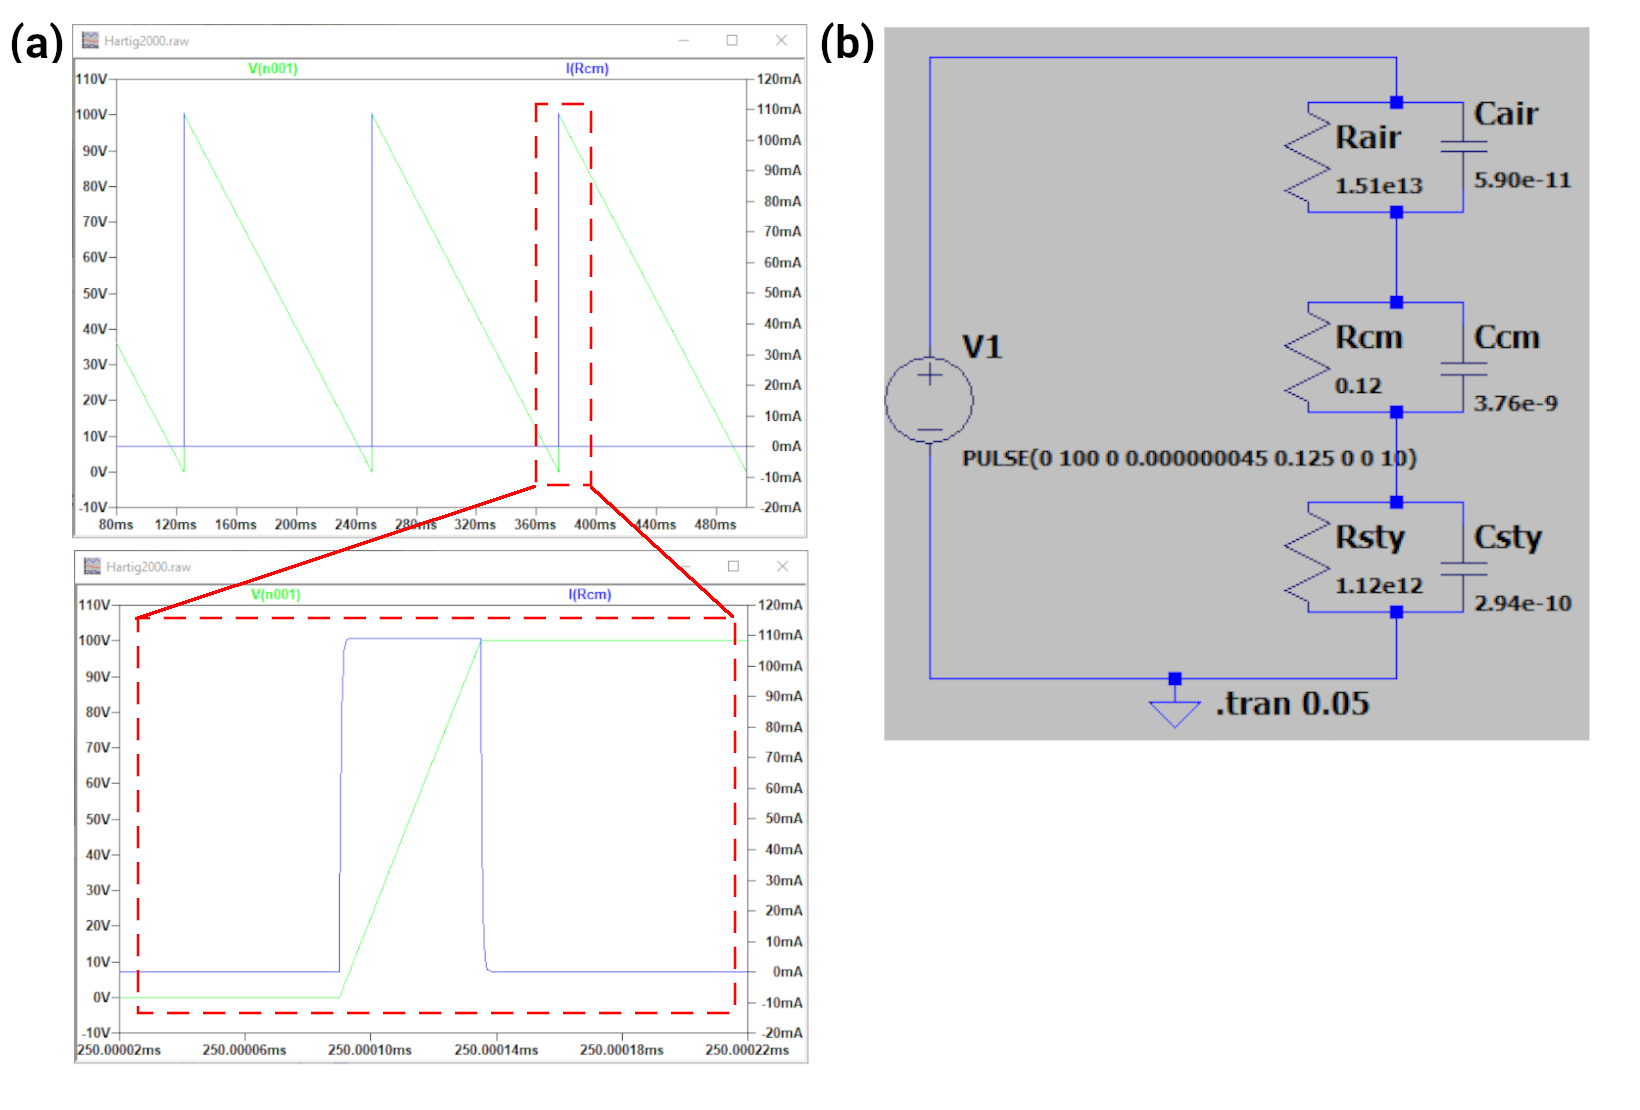
\includegraphics[scale=0.40]{./figures/Figure_5d6.png}}
\caption{Example of LTspice analog circuit simulation for Hartig's et al setup \cite{Hartig2000-ny}. Printscreens from the software environment: (a) digital probe tool visualizer showing the input potential signal (green line) and the electric current peak generated in the culture medium resistor (blue line). The bottom panel shows a detailed view of the rising edge for better visualization of the induced current; (b) the equivalent circuit model of Hartig's setup drawn in LTspice. Abbreviations: R-resistor, C-capacitor, cm-culture medium, sty-polystyrene, V1-voltage source.}
\label{fig5d6}
\end{figure}


\noindent \textit{Selection of studies and theoretical validation.} A bibliographic search was performed on ScienceDirect, Pubmed, and Scopus databases to identify experimental studies using \acs{CCoupled} stimulation. In order to narrow the search, only bone cell lineages were considered for this analysis, taking into consideration our research group's interest in bone tissue engineering. The following search sentence and keywords were considered:"(capacitive stimulation) AND (bone OR osteogenic OR osteogenesis) AND (in vitro)", originating a total of 922 records, 881 in ScienceDirect, 30 in Pubmed, and 11 in Scopus. After the removal of duplicates, the remaining 883 records were screened considering the following exclusion (e) and inclusion (i) criteria:

\begin{itemize}
\footnotesize
\item[(e1)] Publications consisting of reviews or studies \textit{in vivo}, or involving implants or prosthetic devices;
\item[(e2)] Studies targeting biological tissues other than bone;
\item[(e3)] Studies targeting cellular processes other than proliferation and differentiation;
\item[(e4)] Studies using stimulation phenomena other than capacitive coupling;
\item[(i1)] The geometry of the experimental setup and voltage waveform must be reported in sufficient detail to allow the construction of a reasonably accurate model; 
\item[(i2)] The cell culture chamber must be empty of any construct and contain only cellular content and culture medium;
\item[(i3)] The E-Field in the culture medium, measured or estimated, must be reported to allow a comparison with our model's predictions.
\end{itemize}

A total of 16 records fulfilled all criteria. 4 additional records fulfilling all criteria were found by hand searching the reference lists in the 16 records mentioned previously. Eight different setups for capacitive stimulation are reported in these 20 records. They are listed below and were named after the first author of the oldest reference.

\begin{itemize}
\footnotesize
\item  Rodan \textit{et al.}, 1978, original description of this setup \cite{Rodan1978-yu};
\item  Korenstein \textit{et al.}, 1984, original description of this setup \cite{Korenstein1984-qb}, also used in \cite{Laub1984-qm, Danon1984-eu, Binderman1985-mh, Ozawa1989-uz};
\item  Fitzsimmons \textit{et al.}, 1986, original description of this setup \cite{Fitzsimmons1986-ks}, also used in \cite{Fitzsimmons1989-zj, Fitzsimmons1992-vw}; 
\item  Brighton \textit{et al.} 1992, original description of this setup \cite{Brighton1992-gg}, also used in \cite{Armstrong1988-ob, Wang2006-hx, Brighton2008-rl, Clark2014-sz};
\item  Hartig \textit{et al.}, 2000, original description of this setup \cite{Hartig2000-ny}, also used in \cite{Wiesmann2001-uh};
\item  Griffin \textit{et al.}, 2011, original description of this setup \cite{Griffin2011-bb}, also used in \cite{Griffin2013-wp};
\item  Stephan \textit{et al.}, 2020, original description of this setup \cite{Stephan2020-qh};
\item  Khaw \textit{et al.}, 2021, original description of this setup \cite{Khaw2021-tv};
\end{itemize}

\noindent In all these studies, the \acs{EF} values reported were calculated, not measured.

For each one of these setups, the \acs{EF} in the culture medium was calculated using the three approaches described in the previous section. The analytical solutions were implemented in Matlab and Python. The use of LTspice is exemplified in Fig. \ref{fig5d6} with the asymmetric sawtooth voltage waveform applied in Hartig's setup \cite{Hartig2000-ny}. Rodan’s \cite{Rodan1978-yu}, Stephan's \cite{Stephan2020-qh}, and Khaw's \cite{Khaw2021-tv} setups are clearly different from the ideal layered cylindrical geometry. For these setups, a realistic geometry was implemented in COMSOL. Fig. \ref{fig5d7} shows the realistic model for Rodan's setup \cite{Rodan1978-yu}, together with the layered cylindrical model with similar dimensions for analytical and circuit simulator calculations.


\begin{figure}
\makebox[\textwidth][c]{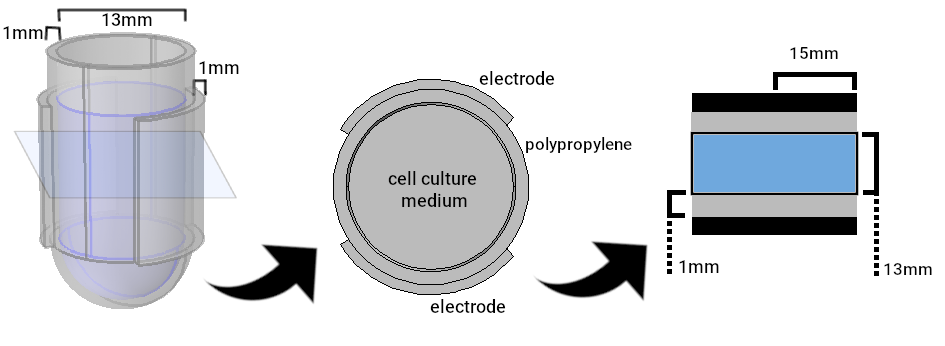
\includegraphics[scale=1.5]{./figures/Figure_5d7.png}}
\caption{\acs{3D} \acs{FEM} model created to replicate Rodan's et al. setup \cite{Rodan1978-yu} and the geometrical approximation considered for its equivalent electronic circuit model.}
\label{fig5d7}
\end{figure}




\section{Results}




\subsection{Scaffold insertion effects}

\noindent \textit{Validation of Brighton \acs{3D} \acs{FEM} model.} Brighton \textit{et al.} \cite{Armstrong1988-ob, Brighton1992-gg} reported that, with their experimental setup (performed in the absence of any scaffold structure) and using a 60 \si{\kilo\hertz} sinusoidal wave of  44.81 \si{\volt} amplitude, they were able to generate an electric field of 20 \si{\milli\volt\per\centi\meter} (2.0 \si{\volt\per\meter}) and a current density of 300 \si{\micro\ampere\per\square\centi\meter} (3.0 \si{\ampere\per\square\meter}). Our \acs{3D} \acs{FEM} model without scaffold predicts an average \acs{EF} of 2.1 \si{\volt\per\meter} and an average current density of 3.2 \si{\ampere\per\square\meter}  in the culture medium. Thus, by comparison, we can conclude that this \acs{3D} \acs{FEM} model accurately predicts the values obtained experimentally in Brighton \textit{et al.} \cite{Armstrong1988-ob, Brighton1992-gg} considering a chamber filled with culture medium and in the absence of a scaffold structure. \hfill \break

\noindent \textit{Sensitivity Analysis.} The sensitivity analysis was performed on the results obtained for Brighton's setup, including the scaffold structure. Sensitivity analysis results from the Delta Moment-Independent Measure are shown in Table \ref{table_delta}. The higher the First Order significance, the greater the contribution of the corresponding parameter to the variation of the electric field magnitude. As expected, in the external \acs{ROI}, the conductivity of the culture medium has the greatest impact on the electric field. Conversely, in the internal \acs{ROI}, the scaffold's conductivity has the greatest impact, followed by the conductivity of the culture medium.


\begin{table}
\caption{ Delta Moment-Independent Measure Results.}
\bigskip
\small
\centering
\begin{tabularx}{405px}{l c c c c c} \toprule[0.15em]
\textbf{ROI} & \textbf{parameter} & \textbf{delta} & \textbf{confidence} & \textbf{1st order significance} & \textbf{ confidence} \\ \cmidrule(l){1-6}
EXTERNAL & $\sigma_{cm}$ &  0.58 & 0.02 & 0.64 & 0.04 \\
& $\epsilon_{cm}$ & 0.28 & 0.01 & 0.17 & 0.01\\
& $\sigma_{s}$  & 0.09 & 0.01 & 0.09 & 0.05\\
& $\epsilon_{s}$ & 0.28 & 0.01 & 0.17 & 0.01 \\ \cmidrule(l){1-6}
INTERFACE & $\sigma_{cm}$ &  0.51 & 0.02 & 0.63 & 0.06 \\
& $\epsilon_{cm}$ & 0.20 & 0.01 & 0.09 & 0.01\\
& $\sigma_{s}$  & 0.40 & 0.03 & 0.68 & 0.03\\
& $\epsilon_{s}$ & 0.20 & 0.01 & 0.09 & 0.01 \\ \cmidrule(l){1-6}
INTERNAL & $\sigma_{cm}$ &  0.39 & 0.02 & 0.45 & 0.04 \\
& $\epsilon_{cm}$ & 0.13 & 0.01 & 0.04 & 0.01\\
& $\sigma_{s}$  & 0.53 & 0.03 & 0.84 & 0.03\\
& $\epsilon_{s}$ & 0.13 & 0.01 & 0.04 & 0.01 \\ \bottomrule[0.15em]
\end{tabularx}
\label{table_delta}
\end{table}


Sensitivity analysis on \acs{FEM} solutions from the parametric sweep study were plotted and grouped by color code in Figure \ref{fig5d8}, with different colors representing different electrical conductivities of the culture medium. Each row shows plots of the average, maximum, and minimum \acs{EF} magnitude in one of the three \acs{ROI}s as a function of the electrical conductivity of the scaffold. Variations in the relative permittivities of the culture medium and scaffold had no noticeable impact on the \acs{EF}. Hence, a single point in these graphs represents the value of the \acs{EF} for all values of the permittivities.


\begin{figure}
\makebox[\textwidth][c]{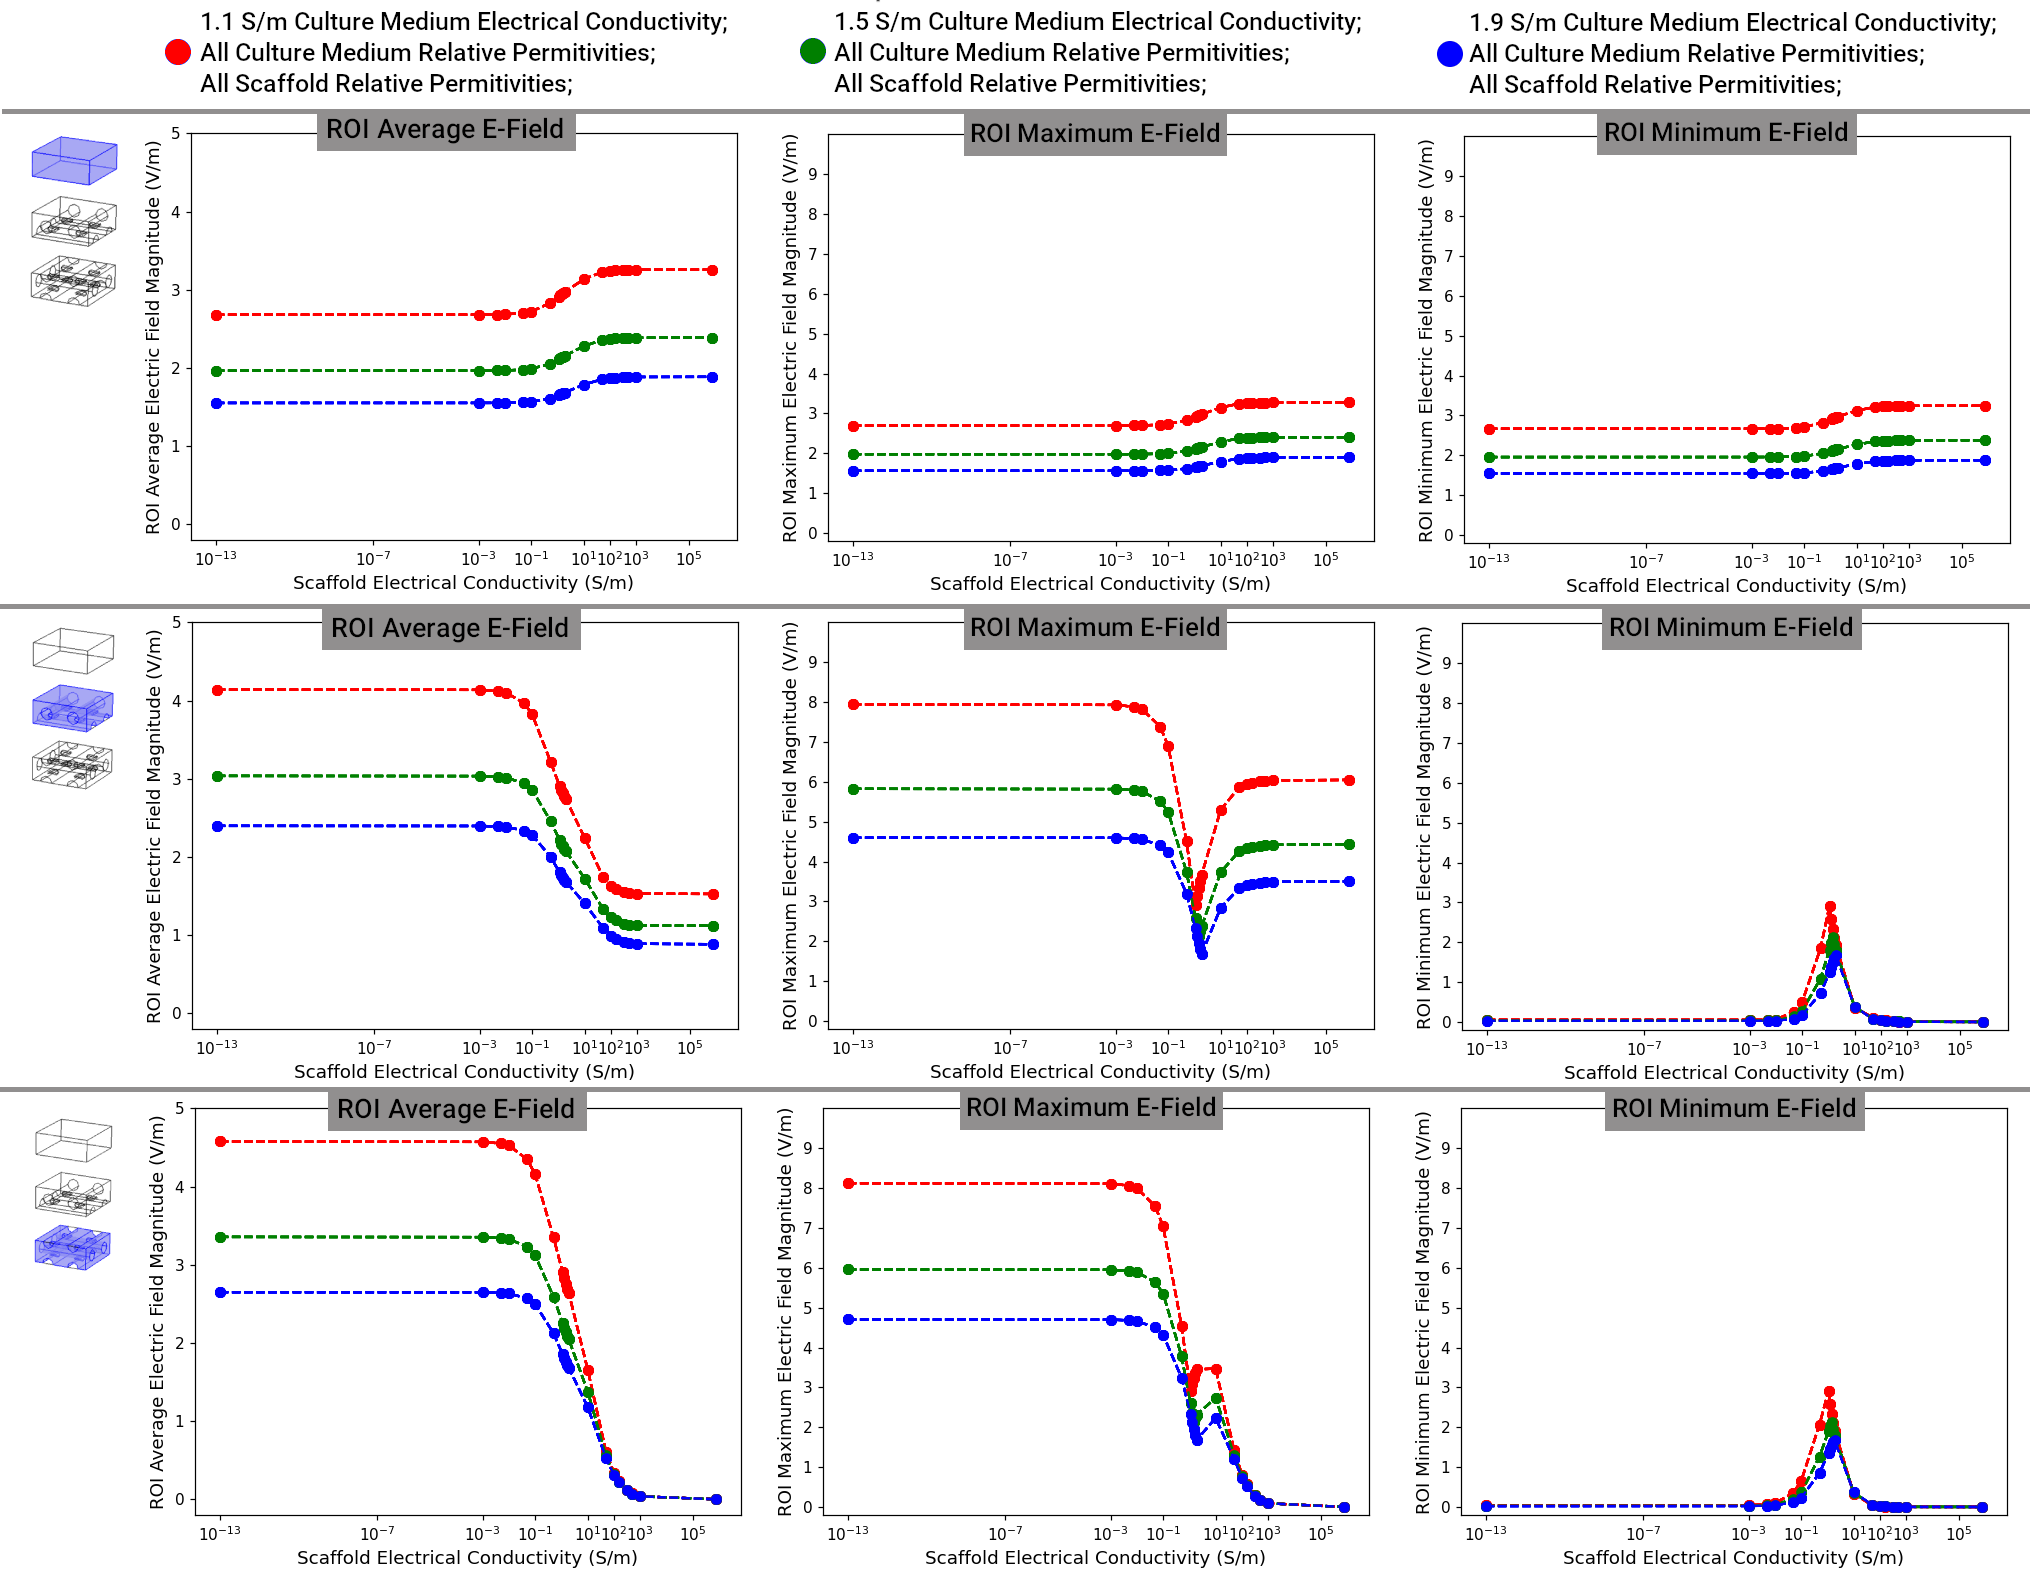
\includegraphics[scale=1.0]{./figures/Figure_5d8.png}}
\caption{One-at-a-time sensitivity analysis of the electric field magnitude per region-of-interest. Each row contains plots for the average, maximum, and minimum electrical field versus the scaffold material's electrical conductivity. Each plot contains all 540 different solutions (each solution is represented by one point), and data are color-coded by culture medium electrical conductivity. The plotted data under analysis only contains solutions from the culture medium nodes.}
\label{fig5d8}
\end{figure}


\noindent We can observe that at 60 \si{\kilo\hertz} the parameters that most influence the magnitude of the \acs{EF} in a bioreactor are the electrical conductivities of both the culture medium and the scaffold material. All plots in Figure \ref{fig5d8} analysis may be split into three regions: one region corresponding to insulating materials with electrical conductivity lower than \num{1.0d-2} \si{\siemens\per\meter}, where changes in scaffold electrical conductivity generate small variations in the \acs{EF}, for a fixed cell culture medium conductivity; another region corresponding to conductive materials with electrical conductivity greater than \num{1.0d2} \si{\siemens\per\meter}, where changes in scaffold electrical conductivity generate small variations in the \acs{EF}; and a transition region, where an almost linear relation between scaffold electrical conductivity and the \acs{EF} magnitude can be observed in the average plots (left column of Figure \ref{fig5d8}). On the other hand, in the maximum and minimum plots, local minima and maxima arise when the electrical conductivity of the scaffold matches that of the cell culture medium (see Figure \ref{fig5d8}). \hfill \break


\noindent \textit{Spatial Distribution Analysis.} Spatial distributions of the \acs{EF} magnitude are presented in Figure \ref{fig5d9}. As expected, the control scaffold, which was considered with the same electrical properties as the cell culture medium, introduces no changes in the predicted \acs{EF}, which remains uniform (Figure \ref{fig5d9} - A1, B1, C1, H1). When the scaffold is more insulating or more conductive than the cell culture medium, the \acs{EF} distribution is greatly affected. A more insulating scaffold material generates local hot zones and cold zones inside the scaffold (Figure \ref{fig5d9} - A2, B2, C2, H2, A3, B3, C3, H3). A more conductive scaffold material shields the surrounding culture medium from the external \acs{EF} stimulation (Figure \ref{fig5d9} - A4, B4, C4, H4). The histograms in the bottom row show that the presence of insulating scaffolds spreads the range of the delivered \acs{EF} magnitude, while the presence of conductive scaffolds reduces this range.


\begin{sidewaysfigure}
\makebox[\textwidth][c]{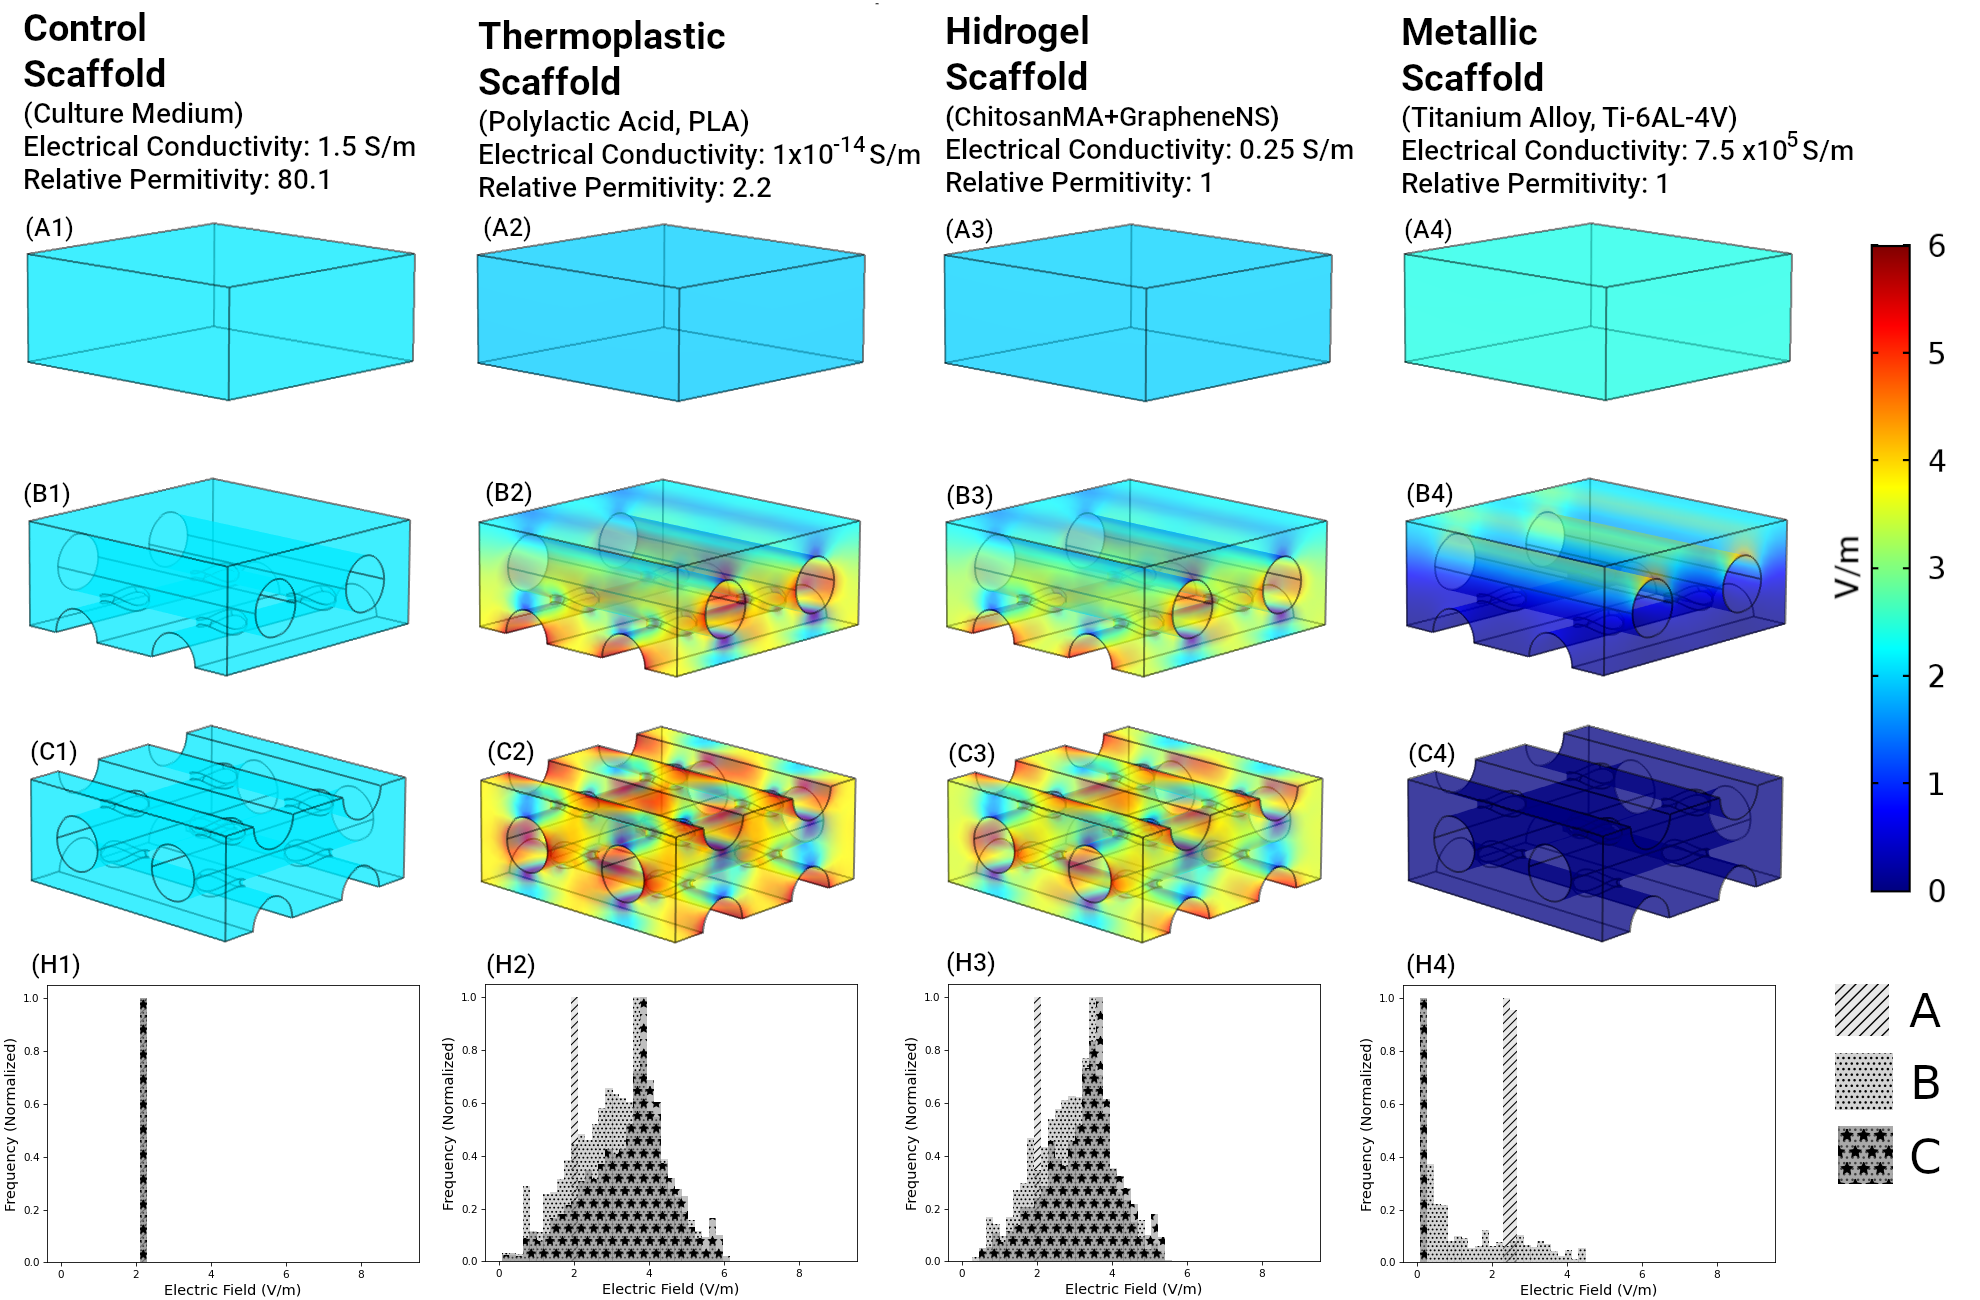
\includegraphics[scale=1.0]{./figures/Figure_5d9.png}}
\caption{Spatial distribution of the \acs{EF} under fixed culture medium electrical parameters ($\sigma$: \num{1.5} \si{\siemens\per\meter}, $\epsilon_r$: 80.1) and fixed external electric stimulation (Brighton's conditions). Each column of the figure presents the predicted result for the specified scaffold material at the \acs{ROI}s labeled from A to C. A normalized frequency histogram of the \acs{EF} magnitude is presented in the bottom row.}
\label{fig5d9}
\end{sidewaysfigure}


\newpage
\subsection{Modelling \acs{CCoupled} reported setups}


Modelling data like the dimensions of the setup, the values of the electrical properties of the materials, and details of the voltage waveform for all eight studies are compiled in Table \ref{table_prop}. Note that the inverse of resistivity, i.e., the conductivity, $\sigma$, is listed in this table. Reasonable estimates for missing values were obtained from the literature presented in the table. The resistance, capacitance, and reactance of the three central layers of each setup were calculated based on these values and are also listed in Table \ref{table_electro}. Khaw's setup is not listed in this table because, at zero frequency, the capacitive reactance of the insulators is infinite (Equation \ref{eqCimpedance}), so the current through the setup and hence the \acs{EF} in the culture medium will be zero.


\begin{table}[p]
\caption{Dimensions, materials electrical properties, and waveforms for each of the setups modeled. $\epsilon_{r}$ represents the relative permittivity, whereas $\sigma$ represents the electric conductivity.}
\bigskip
\tiny
\centering
\begin{tabularx}{\textwidth}{l l l l} \toprule[0.15em]
\textbf{Setup} & \textbf{Dimensions} & \textbf{Materials and Electrical Properties} & \textbf{Waveform} \\ \cmidrule(l){1-4}

Rodan \textit{et al.}, & radius: 15\si{\milli\meter} & \textit{layers 1,4:} 	& Positive trapezoidal pulse,\\
1978 \cite{Rodan1978-yu} & \textit{layers 1,4:} thickness - 1 \si{\milli\meter} & Copper: $\epsilon_{r}$=1; $\sigma$=5.998e7 S/m & 1750 \si{\volt} amplitude,\\
& \textit{layer 2:} thickness - 1 \si{\milli\meter} & \textit{layer 2:} & 0.1 \si{\second} pulse width,\\
& \textit{layer 3:} thickness - 13 \si{\milli\meter} & Polypropylene: $\epsilon_{r}$=2.1; $\sigma$=1e-16 S/m \cite{IneosPP} & 1.85 \si{\milli\second} fall/rise time \\
&  & \textit{layer 3:} &\\
&  & Culture Medium: $\epsilon_{r}$=80.1; $\sigma$=1.5 S/m \cite{Visone2018-sa} & \\ \cmidrule(l){1-4}


Korenstein \textit{et al.}, & radius: 27 \si{\milli\meter} & \textit{layers 1,5:} & \\
 1984 \cite{Korenstein1984-qb} & \textit{layers 1,5:} thickness - 1 \si{\milli\meter} &  Copper: $\epsilon_{r}$=1; $\sigma$=\num{5.99d7} \si{\siemens\per\meter} & Negative trapezoidal pulse, \\
& \textit{layer 2:} thickness - 1.25 \si{\milli\meter} & \textit{layer 2:}  & 300 \si{\volt}, 500 \si{\volt}  \\
& \textit{layer 3:} thickness - 2.25 \si{\milli\meter} &  Air: $\epsilon_{r}$=1.005; $\sigma$=\num{1.0d-14} \si{\siemens\per\meter} & and 1300 \si{\volt} amplitude, \\
& \textit{layer 4:} thickness - 1 \si{\milli\meter} & \textit{layer 3:} &25 \si{\micro\second} pulse width, \\
& & Culture Medium: $\epsilon_{r}$=74; $\sigma$=\num{1.5} \si{\siemens\per\meter} \cite{Korenstein1984-qb, Visone2018-sa} &  7 \si{\nano\second} fall/rise time \\
&  & \textit{layer 4:} & \\
& & Polystyrene: $\epsilon_{r}$=2.5; $\sigma$=\num{6.7d-14} \si{\siemens\per\meter} \cite{Qi2011-se} & \\ \cmidrule(l){1-4}


Fitzsimmons \textit{et al.},  & radius: 26\si{\milli\meter} & \textit{layers 1,5:} & \\
1985 \cite{Fitzsimmons1986-ks} & \textit{layers 1,5:}  thickness - 1 \si{\milli\meter} & Metal Plates: $\epsilon_{r}$=1; $\sigma$=\num{5.99d7} \si{\siemens\per\meter} & Sinusoidal wave, \\
& \textit{layer 2:} thickness - 10 \si{\milli\meter} & \textit{layer 2:} & 10 \si{\volt} amplitude, 10 \si{\hertz} \\
& \textit{layer 3:} thickness - 7 \si{\milli\meter} & Air: $\epsilon_{r}$=1.005; $\sigma$=\num{1.0d-14} \si{\siemens\per\meter} \cite{Seran2017-qg} & \\
& \textit{layer 4:} thickness - 3 \si{\milli\meter} & \textit{layers 3:} & \\
& & Culture Medium: $\epsilon_{r}$=80.1; $\sigma$=1.5 S/m \cite{Visone2018-sa} & \\
& & \textit{layer 4:} & \\
& & Polystyrene: $\epsilon_{r}$=2.5; $\sigma$=\num{6.7d-14} \si{\siemens\per\meter} \cite{Qi2011-se} & \\ \cmidrule(l){1-4}


Brighton \textit{et al.},  & radius: 16.5 \si{\milli\meter} & \textit{layers 1,5:}  & \\
1992 \cite{Brighton1992-gg} & \textit{layers 1,5:} thickness - 1 \si{\milli\meter} & Stainless Steel: $\epsilon_{r}$=1; $\sigma$=\num{4.032d6} \si{\siemens\per\meter} & Sinusoidal Wave, \\
& \textit{layers 2, 4:} thickness - 0.16 \si{\milli\meter} & \textit{layers 2, 4:} & 44.81 \si{\volt} amplitude,\\
& \textit{layer 3:} thickness - 9.8 \si{\milli\meter} & No.1 Glass Coverslip: $\epsilon_{r}$=6.85; $\sigma$=\num{1d-13} \si{\siemens\per\meter} \cite{Hench1972-el} & 60 \si{\kilo\hertz} \\
&  & \textit{layers 3:} & \\
&  & Culture Medium: $\epsilon_{r}$=80.1; $\sigma$=1.5 \si{\siemens\per\meter} \cite{Visone2018-sa} & \\ \cmidrule(l){1-4}
 

Hartig \textit{et al.}, & radius: 65 \si{\milli\meter} & \textit{layers 1,5:} & \\
2000 \cite{Hartig2000-ny} & \textit{layers 1,5:} thickness - 2 \si{\milli\meter} & High Grade Stainless Steel: $\epsilon_{r}$=1; $\sigma$=\num{0.14d7} \si{\siemens\per\meter} & Asymmetric sawtooth, \\
& \textit{layer 2:} thickness - 2 \si{\milli\meter} & \textit{layer 2:} & 100 \si{\volt} peak-to-peak, 	\\
& \textit{layer 3:} thickness - 2.5 \si{\milli\meter} & Air: $\epsilon_{r}$=1.005;  $\sigma$=\num{1.0d-14} \si{\siemens\per\meter} \cite{Seran2017-qg} & 45 \si{\nano\second} risetime, \\
& \textit{layer 4:} thickness - 1 \si{\milli\meter} & \textit{layer 3:} & 62.5 \si{\milli\second} falltime	\\
& & Culture Medium: $\epsilon_{r}$=80.1;  $\sigma$=1.5 \si{\siemens\per\meter} \cite{Visone2018-sa} & \\
& & \textit{layer 4:} & \\
&  & Polystyrene: $\epsilon_{r}$=2.5;  $\sigma$=\num{6.7d-14} \si{\siemens\per\meter} \cite{Qi2011-se} & \\ \cmidrule(l){1-4}


Griffin \textit{et al.}, & radius: 40 \si{\milli\meter} & \textit{layers 1,5:} & \\
 2011 \cite{Griffin2011-bb} & \textit{layers 1,5:} thickness - 1 \si{\milli\meter} & High Grade Steel: $\epsilon_{r}$=1; $\sigma$=\num{5.99d7} \si{\siemens\per\meter} & Degenerate Wave, \\
& \textit{layer 2:} thickness - 2 \si{\milli\meter} & \textit{layer 2:} & 160 \si{\milli\volt} peak-to peak,\\
& \textit{layer 3:} thickness - 4.7 \si{\milli\meter} &  Air: $\epsilon_{r}$=1.005; $\sigma$=\num{1d-14} \si{\siemens\per\meter} \cite{Seran2017-qg} & 62.5 \si{\milli\second} duration,\\
& \textit{layer 4:} thickness - 1 \si{\milli\meter} & \textit{layer 3:} & 16 \si{\hertz}\\
&  & Culture Medium: $\epsilon_{r}$=80.1; $\sigma$=1.5 \si{\siemens\per\meter} \cite{Visone2018-sa} & \\
&  & \textit{layer 4:} & \\
& & Polystyrene: $\epsilon_{r}$=2.5; $\sigma$=6.7e-14 S/m \cite{Qi2011-se} & \\ \cmidrule(l){1-4}


Stephan \textit{et al.}, & 3D Model, radius: 16 \si{\milli\meter} & \textit{layers 1,5:} & \\
2020 \cite{Stephan2020-qh} & \textit{layers 1,5:} thickness - 0.5 \si{\milli\meter} & Ti6Al4V: $\epsilon_{r}$=1; $\sigma$=\num{5.85d5} \si{\siemens\per\meter} \cite{Mitchell2004-ue} & Sinusoidal Wave, \\
& \textit{layer 2,4:}  thickness - 1 \si{\milli\meter} & \textit{layer 2:} & 1.41 \si{\volt} and \\
& \textit{layer 3:} thickness - 32 \si{\milli\meter} & Polystyrene: $\epsilon_{r}$=2.5; $\sigma$=\num{6.7d-14} \si{\siemens\per\meter} \cite{Qi2011-se} & 0.141 \si{\volt} amplitude, \\
& & \textit{layer 3:} & 60 \si{\kilo\hertz} \\
&  & Culture Medium: $\epsilon_{r}$=80.1 \cite{Visone2018-sa}; $\sigma$=1.6 \si{\siemens\per\meter} & \\ \cmidrule(l){1-4}


Khaw \textit{et al.}, & 3D Model, radius: 15 \si{\milli\meter} & \textit{layers 1,5:} & \\
 2021 \cite{Khaw2021-tv} & \textit{layers 1,5:}  thickness - 1.75 \si{\milli\meter} & Electrode: $\epsilon_{r}$=1; $\sigma$=\num{5.99d7} \si{\siemens\per\meter} & Constant Potential \\
& \textit{layer 2,4:} & \textit{layer 2,4:} & 14.2 \si{\volt} and 28.4 \si{\volt},\\
& thickness - 0.75 \si{\milli\meter} & Plastic: $\epsilon_{r}$=2; $\sigma$=\num{6.7d-14} \si{\siemens\per\meter} \cite{Qi2011-se} & \\
& \textit{layer 3:}  thickness - 19.5 \si{\milli\meter} & \textit{layer 3:} & \\
& & Culture Medium: $\epsilon_{r}$=80; $\sigma$=1.7 \si{\siemens\per\meter} & \\
& \textit{air sphere (3D model only):} & \textit{air sphere (3D model only):} & \\
& radius: 120 \si{\milli\meter} & Air: $\epsilon_{r}$=1; $\sigma$=\num{1d-14} \si{\siemens\per\meter} \cite{Seran2017-qg} & \\ \bottomrule[0.15em]
\end{tabularx}
\label{table_prop}
\end{table}



\begin{table}
\caption{Values of the resistances, capacitances, reactances, and frequencies for the three-layer analog circuit models of the \acs{CCoupled} setups.}
\bigskip
\scriptsize
\centering
\begin{tabularx}{410px}{l l l l l l} \toprule[0.15em]
\textbf{Setup} & \textbf{Layers} &\textbf{ Resistance} &\textbf{Capacitance} &\textbf{Reactance} & \textbf{Frequency} \\ \cmidrule(l){1-6}

Rodan \textit{et al.}, & Layer 1 - Polypropylene & \num{1.41d16} \si{\ohm} & \num{1.31d-11} \si{\farad} &\num{-1.41d8}\si{\ohm} & 86.03 \si{\hertz}** \\
1978  \cite{Rodan1978-yu} & Layer 2 - Culture Medium & \num{12.26} \si{\ohm} & \num{3.86d-11} \si{\farad}	&\num{-4.80d7}\si{\ohm} & \\
& Layer 3 - Polypropylene & \num{1.41d16} \si{\ohm} & \num{1.31d-11} \si{\farad} &\num{-1.41d8}\si{\ohm} & \\ \cmidrule(l){1-6}

Korenstein \textit{et al.}, & Layer 1 - Air & \num{5.46d13} \si{\ohm} & \num{1.63d-11} \si{\farad} &\num{-4.29d2}\si{\ohm} & 22.7 \si{\mega\hertz}**	\\
1984 \cite{Korenstein1984-qb} & Layer 2 - Culture Medium & \num{0.65} \si{\ohm} & \num{6.67d-10} \si{\farad} &\num{-0.10d2}\si{\ohm} & \\
& Layer 3 - Polystyrene & \num{6.52d12} \si{\ohm} & \num{5.07d-11} \si{\farad} &\num{-1.38d2}\si{\ohm} & \\ \cmidrule(l){1-6}

Fitzsimmons \textit{et al.}, & Layer 1 - Air & \num{4.71d14} \si{\ohm} & \num{1.89d-12} \si{\farad}	&\num{-8.42d9}\si{\ohm} & 10 \si{\hertz} \\
1985 \cite{Fitzsimmons1986-ks} & Layer 2 - Culture Medium & \num{2.20} \si{\ohm} & \num{2.15d-10} \si{\farad} &\num{-7.40d7} \si{\ohm} & \\
& Layer 3 - Polystyrene & \num{2.11d13} \si{\ohm} & \num{1.57d-11} \si{\farad} &\num{-1.02d9}\si{\ohm} & \\ \cmidrule(l){1-6}

Brighton \textit{et al.}, & Layer 1 - No.1 Glass Coverslip & \num{1.87d12} \si{\ohm} & \num{3.24d-10} \si{\farad} &\num{-8.18d3} \si{\ohm} & 60 \si{\kilo\hertz} \\
1992  \cite{Brighton1992-gg} & Layer 2 - Culture Medium & \num{7.79} \si{\ohm} & \num{6.07d-11} \si{\farad} &\num{-4.37d4}\si{\ohm} & \\
& Layer 3 - No.1 Glass Coverslip & \num{1.87d12} \si{\ohm} & \num{3.24d-10} \si{\farad} &\num{-8.18d3}\si{\ohm}	& \\ \cmidrule(l){1-6}

Hartig \textit{et al.}, & Layer 1 - Air & \num{1.51d13} \si{\ohm} & \num{5.91d-11} \si{\farad}	&\num{-7.62d2}\si{\ohm} & 3.5 \si{\mega\hertz}** \\
2000 \cite{Hartig2000-ny} & Layer 2 - Culture Medium & \num{0.13} \si{\ohm} & \num{3.76d-09} \si{\farad} &\num{-1.20d1}\si{\ohm} & \\
& Layer 3 - Polystyrene & \num{1.12d12} \si{\ohm} & \num{2.94d-10} \si{\farad} &\num{-1.53d2}\si{\ohm} & \\ \cmidrule(l){1-6}

Griffin \textit{et al.}, & Layer 1 - Air & \num{3.98d13} \si{\ohm} & \num{2.24d-11} \si{\farad}	&\num{-3.23d8}\si{\ohm} & 22 \si{\hertz} \\
 2011 \cite{Griffin2011-bb} & Layer 2 - Culture Medium & \num{0.62}  \si{\ohm} & \num{7.58d-10} \si{\farad}	&\num{-9.54d6}\si{\ohm} & \\
& Layer 3 - Polystyrene & \num{2.97d12} \si{\ohm} & \num{1.11d-10} \si{\farad} &\num{-6.50d7}\si{\ohm} & \\ \cmidrule(l){1-6}

Stephan \textit{et al.}, & Layer 1 - Polystyrene & \num{1.86d13} \si{\ohm} & \num{1.78d-11} \si{\farad} &\num{-1.49d5}\si{\ohm} & 60 \si{\kilo\hertz} \\
2020 \cite{Stephan2020-qh} & Layer 2 - Culture Medium & \num{24.87} \si{\ohm} & \num{1.78d-11} \si{\farad}	&\num{-1.49d5}\si{\ohm} & \\
& Layer 3 - Polystyrene & \num{1.86d13} \si{\ohm} & \num{1.78d-11} \si{\farad} &\num{-1.49d5}\si{\ohm} & \\ \bottomrule[0.15em]
\multicolumn{6}{r}{** Matched frequency}\\
\end{tabularx}
\label{table_electro}
\end{table}


The comparisons between the values of the \acs{EF} in the culture medium reported in the original papers and those obtained using the three approaches described in the methods section are listed in Tables \ref{tab_agree} and \ref{tab_disagree}. Table \ref{tab_agree} shows that there is a good agreement between the originally reported values and our theoretical estimates in the case of the studies by Brighton \textit{et al.} \cite{Brighton1992-gg}, Hartig \textit{et al.} \cite{Hartig2000-ny} and Stephan \textit{et al.} \cite{Stephan2020-qh}. In Brighton’s study \cite{Brighton1988-vc}, the reported \acs{EF} values obtained using analytical and \acs{FEM} approaches agree with our estimates for the two frequencies and applied voltages considered. The results are consistent with the fact that the \acs{EF} is proportional to the applied voltage and that it is (approximately) proportional to the frequency. Hartig \textit{et al.} reported a potential difference of 100 \si{\micro\volt} across the cell monolayer. We assumed that the thickness of the monolayer was 25 \si{\micro\meter} as typically reported in the literature \cite{Ge2014-mj}, which yielded an \acs{EF} estimate of 4 \si{\volt\per\meter}. We also had to assume a risetime of 45 \si{\nano\second} for the asymmetric sawtooth voltage waveform, based on the specifications sheet of the function generator Hameg HM1881-2. \footnote{www.farnell.com/datasheets/318574.pdf} Given these and other uncertainties, the agreement between the reported value (4.0 \si{\volt\per\meter}) and our predictions (5.5 \si{\volt\per\meter}) is acceptable. Stephan \textit{et al.} \cite{Stephan2020-qh} estimated the \acs{EF} strength in a 3D model of a single well using the \acs{FEM} approach. Since the authors did not report the thickness of the petri dish wall, which separates the electrodes from the cell culture medium, we assumed a typical wall thickness of 1 \si{\milli\meter}. Despite this uncertainty, a good agreement between our predictions and the reported \acs{EF} values was found. In general, the small differences found in our predictions might be attributed to some of the model parameters not being described exactly in the original studies. Also, note that our three numerical approaches yield the same results, as expected.



\begin{table}
\caption{List of studies where an agreement was observed between the reported and predicted magnitude of the \acs{EF} in the culture medium.}
\bigskip
\footnotesize
\centering
\begin{tabularx}{405px}{l l l} \toprule[0.15em]
\multicolumn{3}{l}{Brighton \textit{et al.}, 1992 \cite{Brighton1992-gg} original setup, also reused in \cite{Armstrong1988-ob, Wang2006-hx, Brighton2008-rl, Clark2014-sz}}\\ \cmidrule(l){1-3}
\textbf{Waveform: sinusoidal} & \textbf{60 \si{\kilo\hertz}, \textbf{44.81 \si{\volt} amplitude}} & \textbf{10 \si{\hertz}, \textbf{1.33 \si{\volt} amplitude}} \\
Reported Value & 2.0 \si{\volt\per\meter} & \num{1.0d-5} \si{\volt\per\meter} \\
\textit{Equivalent Electronic Circuit:} & & \\
- Analytical & 2.1 \si{\volt\per\meter} & \num{1.0d-5} \si{\volt\per\meter} \\
- LTspice (real waveform) & 2.1 \si{\volt\per\meter} & \num{1.0d-5} \si{\volt\per\meter} \\
Finite Element Analysis (FEA) & 2.1 \si{\volt\per\meter} & \num{1.0d-5} \si{\volt\per\meter} \\ \cmidrule(l){1-3}


\multicolumn{3}{l}{Hartig \textit{et al.}, 2000 \cite{Hartig2000-ny} original setup, also reused in \cite{Wiesmann2001-uh}}\\ \cmidrule(l){1-3}
\textbf{Waveform: asymmetric sawtooth} &\multicolumn{2}{l}{\textbf{45 \si{\nano\second} rise-time}, matched frequency 3.5 \si{\mega\hertz}, 100 \si{\volt} pk-pk} \\
Reported Value &\multicolumn{2}{l}{4 \si{\volt\per\meter}} \\
\textit{Equivalent Electronic Circuit:} &\multicolumn{2}{l}{} \\
- Analytical &\multicolumn{2}{l}{5.5 \si{\volt\per\meter}}	\\
- LTspice (real waveform) &\multicolumn{2}{l}{5.5 \si{\volt\per\meter}} \\
Finite Element Analysis (FEA) &\multicolumn{2}{l}{5.5 \si{\volt\per\meter}} \\ \cmidrule(l){1-3}


\multicolumn{3}{l}{Stephan \textit{et al.}, 2020 \cite{Stephan2020-qh} original setup}\\ \cmidrule(l){1-3}
\textbf{Waveform: sinusoidal} &\textbf{60 \si{\kilo\hertz}, 0.141\si{\volt} amplitude} & \textbf{60 \si{\kilo\hertz}, 1.41\si{\volt} amplitude} \\
Reported Value &(\num{2.5}-\num{3.5})x\num{d-4} \si{\volt\per\meter}	&(\num{2.5}-\num{3.5})x\num{d-3} \si{\volt\per\meter}\\
\textit{Equivalent Electronic Circuit:} & & \\
- Analytical & \num{3.7d-4} \si{\volt\per\meter} & \num{3.7d-3} \si{\volt\per\meter} \\
- LTspice (real waveform) & \num{3.7d-4} \si{\volt\per\meter} & \num{3.7d-3} \si{\volt\per\meter} \\
Finite Element Analysis (FEA) &(\num{2.2}-\num{6.0})x\num{d-4} \si{\volt\per\meter} & (\num{2.5}-\num{3.5})x\num{d-3} \si{\volt\per\meter} \\ \bottomrule[0.15em]
\end{tabularx}
\label{tab_agree}
\end{table}


 Table \ref{tab_disagree} shows the results concerning the studies where a discrepancy between the reported values and our estimates was observed. In all cases, the \acs{EF} in the culture medium was overestimated. In Rodan \textit{et al.} \cite{Rodan1978-yu}, no information on how the \acs{EF} was estimated is provided. However, the slow risetime of 1.85 \si{\milli\second}, which corresponds to a matched frequency of 86 \si{\hertz}, seemed too low to produce an \acs{EF} of \num{1.2d5} \si{\volt\per\meter}. As the setup's geometry differs from the layered cylindrical setup, a realistic model was implemented in COMSOL, as shown in Figure \ref{fig5d7}. A layered cylindrical setup with similar dimensions was also designed to calculate resistances and capacitances for use in the analytical and circuit simulator approaches. All numerical approaches converged to a predicted field of about \num{6.0d-3} \si{\volt\per\meter}, which is more than 7 orders of magnitude below the reported value. Interestingly, the values obtained with the analytical and circuit simulator approaches are very similar to the values predicted by the \acs{FEM} analysis, even though they are based on different geometries.


\begin{table}
\caption{List of studies where a disagreement was observed between the reported and predicted magnitude of the \acs{EF} in the culture medium.}
\bigskip
\footnotesize
\centering
\begin{tabularx}{405px}{l l l l} \toprule[0.15em]
\multicolumn{4}{l}{Rodan \textit{et al.}, 1978 \cite{Rodan1978-yu} original setup}\\ \cmidrule(l){1-4}
\textbf{Waveform: trapezoidal} & \multicolumn{3}{l}{\textbf{1.85 \si{\milli\second} rise-time}, matched freq. 86 \si{\hertz}, 1750 \si{\volt} amplitude} \\
Reported Value &\multicolumn{3}{l}{\num{1.2d5} \si{\volt\per\meter}} \\
\textit{Equivalent Electronic Circuit:} &\multicolumn{3}{l}{} \\
- Analytical &\multicolumn{3}{l}{\num{5.9d-3} \si{\volt\per\meter}} \\
- LTspice (real waveform) &\multicolumn{3}{l}{\num{5.9d-3}\si{\volt\per\meter}} \\
Finite Element Analysis (FEA) &\multicolumn{3}{l}{\num{6.0d-3} \si{\volt\per\meter}} \\ \cmidrule(l){1-4}


\multicolumn{4}{l}{Korenstein \textit{et al.}, 1984 \cite{Korenstein1984-qb} original setup, also reused in \cite{Laub1984-qm, Danon1984-eu, Binderman1985-mh, Ozawa1989-uz}}\\ \cmidrule(l){1-4}
\textbf{Waveform: trapezoidal} &\multicolumn{3}{l}{\textbf{7 \si{\nano\second} rise-time}, matched freq. 22.7 \si{\mega\hertz},} \\
&300 \si{\volt} amplitude & 500 \si{\volt} amplitude & 1300 \si{\volt} amplitude \\
Reported Value &\num{1.3d3} \si{\volt\per\meter} &\num{2.2d3} \si{\volt\per\meter}	&\num{5.4d3} \si{\volt\per\meter} \\
\textit{Equivalent Electronic Circuit:} & & & \\
- Analytical &\num{1.5d2} \si{\volt\per\meter} &\num{2.6d2} \si{\volt\per\meter} &\num{6.7d2} \si{\volt\per\meter} \\
- LTspice (real waveform) &\num{1.5d2} \si{\volt\per\meter} &\num{2.6d2} \si{\volt\per\meter}	&\num{6.7d2} \si{\volt\per\meter} \\
Finite Element Analysis (FEA) &\num{1.5d2} \si{\volt\per\meter} &\num{2.6d2} \si{\volt\per\meter}	&\num{6.7d2} \si{\volt\per\meter} \\ \cmidrule(l){1-4}


\multicolumn{4}{l}{Fitzsimmons \textit{et al.}, 1985 \cite{Fitzsimmons1986-ks} original setup, also reused in \cite{Fitzsimmons1989-zj, Fitzsimmons1992-vw}}\\ \cmidrule(l){1-4}
\textbf{Waveform: sinusoidal} &\multicolumn{3}{l}{\textbf{10 \si{\hertz}, 10 \si{\volt} amplitude}} \\
Reported Value &\multicolumn{3}{l}{\num{1.0d-5} \si{\volt\per\meter}} \\
\textit{Equivalent Electronic Circuit:} &\multicolumn{3}{l}{} \\
- Analytical &\multicolumn{3}{l}{\num{3.3d-7} \si{\volt\per\meter}} \\
- LTspice (real waveform) &\multicolumn{3}{l}{\num{3.3d-7} \si{\volt\per\meter}} \\
Finite Element Analysis (FEA) &\multicolumn{3}{l}{\num{3.3d-7} \si{\volt\per\meter}} \\ \cmidrule(l){1-4}


\multicolumn{4}{l}{Griffin \textit{et al.}, 2011 \cite{Griffin2011-bb} original setup, also reused in \cite{Griffin2013-wp}}\\ \cmidrule(l){1-4}
\textbf{Waveform: degenerate wave} &\multicolumn{3}{l}{\textbf{Damped oscillation}, matched freq. 22 \si{\hertz}, 100 \si{\milli\volt} amplitude} \\
Reported Value &\multicolumn{3}{l}{\num{10} \si{\volt\per\meter}} \\
\textit{Equivalent Electronic Circuit:} &\multicolumn{3}{l}{} \\
- Analytical &\multicolumn{3}{l}{\num{3.4d-8} \si{\volt\per\meter}} \\
- LTspice (real waveform) &\multicolumn{3}{l}{\num{3.5d-8} \si{\volt\per\meter}} \\
Finite Element Analysis (FEA) &\multicolumn{3}{l}{\num{3.6d-8} \si{\volt\per\meter}} \\ \cmidrule(l){1-4}

\multicolumn{4}{l}{Khaw \textit{et al.}, 2021 \cite{Khaw2021-tv} original setup}\\ \cmidrule(l){1-4}
\textbf{Waveform: Steady Potential} &\multicolumn{3}{l}{\textbf{Constant DC Potential}} \\
&\multicolumn{2}{l}{14.2 \si{\volt} amplitude} & 28.4 \si{\volt} amplitude \\  
Reported Value &\multicolumn{2}{l}{\num{100} \si{\volt\per\meter}} & \num{200} \si{\volt\per\meter} \\
Equivalent Electronic Circuit: &\multicolumn{2}{l}{} & \\
- Analytical &\multicolumn{2}{l}{\num{0} \si{\volt\per\meter}} & \num{0} \si{\volt\per\meter} \\ \bottomrule[0.15em]
\end{tabularx}
\label{tab_disagree}
\end{table}


In Korenstein \textit{et al.} \cite{Korenstein1984-qb}, only the relative permittivity of the various layers was taken into account, and the electric resistivity of the culture medium was not considered. However, the resistance of the culture medium is the dominant factor affecting the E-Field in this layer. The other fundamental parameter that was missing was the risetime of the trapezoidal wave. We assumed a risetime of 7 \si{\nano\second} based on the specifications sheet of the signal generator used (Velonex 380 \footnote{www.testequipmentconnection.com/4603/Velonex$\_$380.php}). This assumption and the ones related to the conductivity of the various layers (Table \ref{table_prop}) lead to an estimate for the \acs{EF} in the culture medium of 154 \si{\volt\per\meter} for an applied voltage of 300 \si{\volt} in the different numerical approaches used. This is one order of magnitude lower than the values reported by Korenstein \textit{et al.} \cite{Korenstein1984-qb}. Estimates of the \acs{EF} for voltages other than 300 \si{\volt} can be derived from the estimate presented here because the field is simply proportional to the applied voltage. In their paper, Korenstein et al. state that several experimental factors related to the electrical circuit distorted the voltage waveform, which suggests that the effective risetime may have been significantly longer than 7 \si{\nano\second}. This would lead to a lower predicted \acs{EF} value.  

The value of the \acs{EF} reported in Fitzsimmons \textit{et al.} (\num{1.0d-5} \si{\volt\per\meter}) \cite{Fitzsimmons1986-ks} also differs significantly from our estimate of \num{3.0d-7} \si{\volt\per\meter}. This discrepancy arises from an incorrect estimate of the resistance of the culture medium: it seems that the resistivity of the culture medium (100 \si{\ohm\centi\meter}) was incorrectly assumed to be equal to its resistance (100 \si{\ohm}). We estimated the resistance of the culture medium to be about 30 times lower, which led to a reduction in the estimated \acs{EF} by the same factor. Also, Fitzsimmons \textit{et al.} did not calculate the total impedance of the setup by summing the complex impedances of the various layers, which also led to a small error in this value.

Griffin \textit{et al.} \cite{Griffin2011-bb} used the same setup as Hartig \textit{et al.} but they did not consider the time-varying nature of the applied voltage, the Degenerate Wave (DW), nor the conductive nature of the culture medium (see \cite{Griffin2013-wp}, supplementary Figure$\_$S1.docx, File$\_$S2.docx). To get an accurate estimate of the field, we obtained values for the conductivity of the various materials from the literature and digitized the DW from Figure 1 in \cite{Griffin2013-wp}. For use in our analytical approach, we estimated that a sine wave with a frequency of 22 \si{\hertz} and 100 \si{\milli\volt} amplitude would have approximately the same maximum rate of change with time as the DW. The amplitude was taken to be 100 \si{\milli\volt} because this is the amplitude of the first (positive) deflection of the DW. Our numerical approaches estimated the \acs{EF} in the culture medium to be approximately \num{3.5d-8} \si{\volt\per\meter}, more than 8 orders of magnitude smaller than the value reported by Griffin \textit{et al.} \cite{Griffin2011-bb}.

Khaw \textit{et al.} \cite{Khaw2021-tv} reported to have applied \acs{EF}s of \num{100} \si{\volt\per\meter} and \num{200} \si{\volt\per\meter} in their capacitively-coupled bioreactor by applying constant potential differences of 14.2 \si{\volt} and 28.4 \si{\volt} respectively. These estimates were obtained with a \acs{FEM} \acs{3D} model, using the electrostatics interface to compute the \acs{EF}. The selected set of equations does not take into account the conservation of currents and Ohm's law, so it is insufficient to correctly model this \acs{CCoupled} setup. As we referred in the methods section, the response of \acs{CCoupled} systems is almost that of a capacitor, so the \acs{EF} generated in the culture medium by continuous \acs{DC} stimulation is effectively zero.




\newpage
\section{Discussion}

Both works presented in this chapter focused their analysis on \acs{CCoupled} systems because they allow to avoid the faradaic products that constitute a significant disadvantage of \acs{DCoupled} systems, while simultaneously avoiding the concurrent application of a magnetic field that characterizes \acs{ICoupled} systems.

The \acs{FEM} analysis results for the scaffold insertion effect show that the scaffold effect in \acs{CCoupled} electric stimulation delivery cannot be ignored. However, different waveforms, with different frequency spectra, will produce changes in the delivered \acs{EF}. It is expected that waveforms with frequencies below the studied 60 \si{\kilo\hertz} will generate lower \acs{EF} magnitudes for the same voltage (44.81 \si{\volt}), but maintain the \acs{EF} spatial patterns shown in Figure \ref{fig5d9}. The effects introduced by the relationship between scaffold conductivity and culture medium conductivity will predictably remain valid for frequencies lower than the studied 60 \si{\kilo\hertz}.

Sensitivity analysis data obtained from the one-at-a-time variation method (Figure \ref{fig5d8}) and by delta moment-independent measures (Table \ref{table_delta}) reveals that permittivities of the scaffold and culture medium have a residual effect on the delivered \acs{EF}. In contrast, the electrical conductivities of the scaffold and culture medium regulate the major effects presented in this work. More insulating scaffolds generate a surrounding \acs{EF} pattern with peaks and troughs, amplifying and attenuating the delivered \acs{EF}. This effect is attributed to the opposition produced by the scaffold to the electric current flow. At the applied frequency, permittivities did not add a noticeable contribution to the resultant \acs{EF}, however, for far higher frequencies, it is expected that the influence of both permittivities on the \acs{EF} surrounding the scaffold becomes more significant. The \acs{EF} pattern is geometry dependent. Hence, scaffolds with different configurations from the orthogonal one studied in this work will present different spatial patterns of \acs{EF}. Patterns generated by different scaffold structures will be further addressed in the next chapter. According to the presented results, scaffolds made of more conductive materials will shield the surrounding culture medium from the externally applied \acs{EF}, delivering a strongly attenuated \acs{EF}, more independent of the scaffold geometry.

According to the literature \cite{Distler2020-gi, Balint2014-ti}, many scaffold materials have electrical conductivity values within the transition region identified in Figure \ref{fig5d8}. This factor, together with the experimental variability of the conductivity of culture media, makes it almost impossible to compare electrical stimulation studies that did not take into account the effect introduced by the scaffold presence in those experimental conditions. This comparison would be decisive in standardizing parameters for stimulation protocols using scaffolds for a specific cellular outcome. 

A recent work from Zimmermann \textit{et al.} \cite{Zimmermann2020-cc} focused on tailoring the electrical conductivity of a hydrogel material used as a cell culture substrate for maximizing the effect on cell \ac{TMP}, also utilizing Brighton's setup and protocol. Their findings are in line with our results, by concluding that hydrogel conductivity plays an important role in the external electrical stimulation effect. The authors observed that the lower conductivity of hydrogel contributes to increasing \acs{TMP} values and that the effect of the hydrogel permittivity on electrical stimulation is negligible. Also, our current work does not address directly the effect on \acs{TMP},  but it does show that lower conductivity materials generate higher \acs{EF}s peaks and troughs in their surroundings, probably contributing also to higher \acs{TMP} values. Our conclusions apply to different classes of materials and include a broader range of electrical conductivities and permittivities. The predicted effects of the scaffold's presence on the induced \acs{EF} reported here must be taken into account when designing and conducting electrical stimulation experimental protocols, as they may strongly influence the outcomes and the understanding regarding the electrical stimulation effectiveness.    


% Outro Artigo

Regarding the comparative analysis of reported \acs{CCoupled} setups regarding their applied \acs{EF} versus the correspondent \acs{FEM} prediction, results found an overestimation of the \acs{EF} in the majority of the works selected for this study. This analysis also identified some wrong assumptions regarding the physics underlying the calculation of the \acs{EF} in the culture medium. Based on these findings, we provide detailed descriptions of different numerical models that calculate the resultant \acs{EF} to guide future applications of \acs{CCoupled} \acs{EF} stimulation in \acs{BTE}. 

In the three studies where there was a good agreement between the reported values and our theoretical estimates, we found that the electrical response of the setup was modeled correctly. Brighton \textit{et al.} \cite{Brighton1992-gg} do not provide detailed information regarding the methods used to estimate the \acs{EF} in the culture medium. However, in \cite{Brighton1988-vc}, they stated in a footnote that “The \acs{EF} and the current density were calculated on a macroscopic continuum basis by solving the boundary value problem constructed from Maxwell’s electromagnetic field equations. Comparable solutions were obtained using a two-dimensional closed-form solution technique and a three-dimensional computer-generated solution using finite element analysis”. This approach is similar to ours, which, together with reasonable estimates of the missing physical parameters, predicted almost the same value for the \acs{EF} as reported in the paper. Hartig \textit{et al.} \cite{Hartig2000-ny} based their \acs{EF} estimates on an electric circuit described in \cite{Wiesmann2001-uh} and that is essentially the same as the one shown in Figure \ref{fig5d6} of this paper. Unfortunately, the values of the resistances and capacitances were not specified, nor was the duration of the rising edge of the saw-tooth voltage waveform. In addition, a potential difference across a cellular monolayer was reported, not the \acs{EF} in the culture medium. Despite these unknowns, the agreement between the reported value and our calculations was good. In Stephan \textit{et al.} \cite{Stephan2020-qh} the \acs{EF} was computed using the electric currents interface of the COMSOL software, based on the quasi-electrostatic approximation of Maxwell's equations. This \acs{FEM} approach is the same as ours and despite the uncertainty due to the absence of the exact petri dish wall thickness, a good agreement was found with a typical value for this missing parameter.

Fitzsimmons \textit{et al.} \cite{Fitzsimmons1986-ks} used an appropriate simplified electrical circuit to model the electrical response of the setup, but the resistance of the culture medium was likely overestimated, leading to an overestimate of the \acs{EF}.

In the studies by Rodan \textit{et al.} \cite{Rodan1978-yu}, Korenstein \textit{et al.} \cite{Korenstein1984-qb}, Griffin \textit{et al.} \cite{Griffin2011-bb} and Khaw \textit{et al.} \cite{Khaw2021-tv} the approach followed to estimate the \acs{EF} was inappropriate because it did not consider the conductive nature of the culture medium or the temporal variation of the applied voltage. In \acs{CCoupled} setups, the electric charge on the electrodes creates an \acs{EF} in the culture medium, which leads to the accumulation of charge of opposite sign at the interface between the (conductive) culture medium and the insulator. This secondary charge distribution creates an \acs{EF} that points in the opposite direction to the \acs{EF} created by the charge on the electrodes and is such that, for a constant applied voltage (\acs{DC}), the total \acs{EF} in the culture medium would be zero. 

In Rodan \textit{et al.} \cite{Rodan1978-yu}, the reported value of \num{1.166d5} \si{\volt\per\meter} was obtained by dividing the applied voltage (1750 \si{\volt}) by the distance between electrodes (15 \si{\milli\meter}) but this is physically incorrect, given that the materials between the electrodes have different conductivities and permittivities. In Korenstein \textit{et al.} \cite{Korenstein1984-qb}, the resistive impedance of the culture medium is considerably lower than its capacitive reactance (see Table \ref{table_electro}), despite the high frequencies involved. It is therefore its resistive impedance that will determine the potential drop and hence the \acs{EF} in the culture medium, thereby invalidating the assumption on which the calculations were based. In Griffin \textit{et al.} \cite{Griffin2011-bb}, the low resistive impedance of the culture medium is also ignored, resulting in an overestimation of the \acs{EF} by eight orders of magnitude. In Khaw \textit{et al.} \cite{Khaw2021-tv}, the choice of the electrostatic interface for the \acs{FEM} analysis, which does not take into account currents in conducting media, is the reason why a non-zero \acs{EF} was wrongly predicted.

The analysis of these eight studies highlights the importance of accurate and detailed reporting of the physical parameters of the setup (dimensions, electrical properties) and the voltage waveform (particularly, risetimes of sharp edges) to enable replication of the electrical stimulation. When this information is available, many numerical approaches can produce sufficiently accurate estimates of the \acs{EF} in the culture medium. The resulting model of the setup has several useful characteristics. It can be shared and used to investigate the effect of changes in the setup parameters and voltage waveform on the \acs{EF} in the culture medium. It can also be used to determine the changes in the setup required to achieve the desired \acs{EF}. For example, \acs{CAD} files are a practical way of documenting and sharing the geometry of the setup.

Regarding the choice of the numerical approach (see Figure \ref{fig5d10}), an analytical solution based on the simple series C-R-C circuit shown in Figure \ref{fig5d3}d should provide a useful first estimate of the \acs{EF} in most cases. This approach can be extended to non-sinusoidal waveforms by estimating the frequency associated with the applied voltage's fastest rising or falling edges. Alternatively, a circuit simulator like LTspice can illustrate the temporal variation of the \acs{EF} in the culture medium for arbitrary waveforms. Note, however, that a single frequency must still be chosen to calculate the capacitance of the insulating layers. Also, a very good approximation to the temporal variation of the \acs{EF} can be obtained by simply plotting the first derivative of the voltage waveform with respect to time (Equation \ref{eqRelation}).

\begin{figure}
\makebox[\textwidth][c]{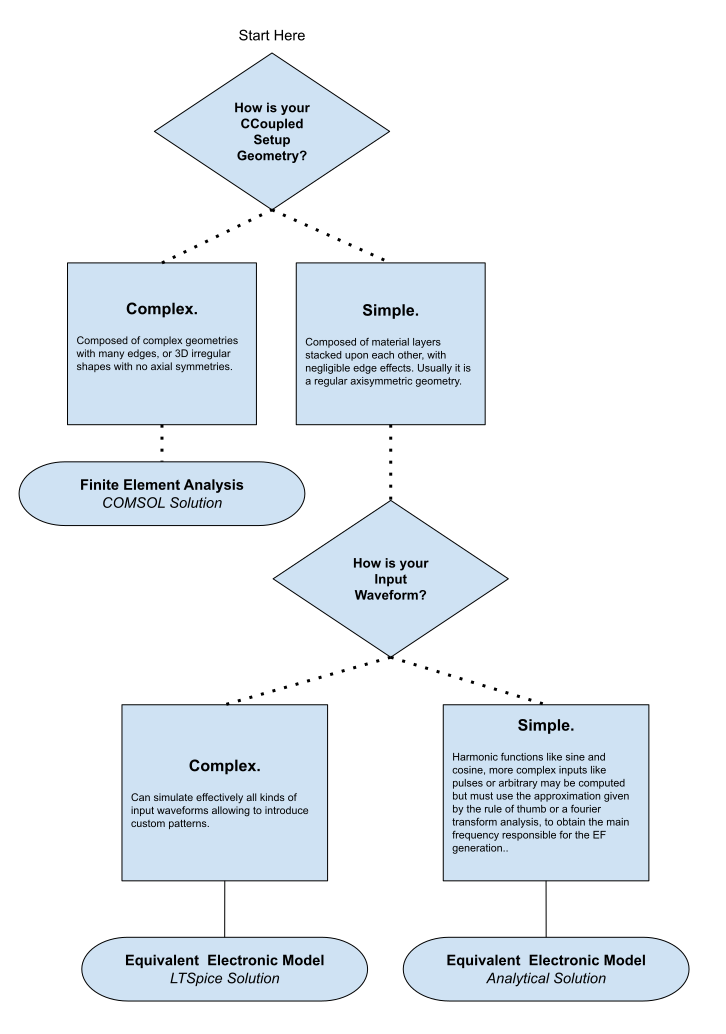
\includegraphics[scale=0.6]{./figures/Figure_5d10.png}}
\caption{Decision flowchart to choose an appropriate numerical modelling approach for a particular CCoupled setup.}
\label{fig5d10}
\end{figure}

If the geometry of the setup differs significantly from the ideal coaxial geometry of the constant section that is assumed in the analytical solution, then the \acs{FEM} method may be used to take into account the complexity of the geometry. However, even in the case of the geometry implemented in Rodan \textit{et al.} \cite{Rodan1978-yu} and shown in Figure \ref{fig5d7}a, it was possible to estimate the \acs{EF} using a simple cylindrical (coaxial) model (Figure \ref{fig5d7}b) and still obtain almost identical values for the \acs{EF} (Table \ref{tab_disagree}). Another advantage of the \acs{FEM} model is that it makes no assumptions about the frequency spectrum of the applied voltage, which is not the case for the analytical and circuit simulator approaches. Nonetheless, our predictions of the \acs{EF} for the eight studies analyzed (Tables \ref{tab_agree} and \ref{tab_disagree}) are practically the same for all three independent approaches (less than 3\% deviation from the mean value between the three prediction methods). 

The \acs{EF} values reported in the selected studies ranged from \num{1.0d-5} \si{\volt\per\meter} to \num{1.0d5} \si{\volt\per\meter}. According to our calculations, the actual range of applied fields was \num{1.0d-8} \si{\volt\per\meter} to \num{1.0d2} \si{\volt\per\meter}, still a range of 10 orders of magnitude. This is explained in part by the wide range of frequencies used, from Hz to MHz, and the fact that \acs{EF} strength is proportional to frequency in the setups described.

The effect of electrical stimulation on cell response is likely to be frequency-dependent. For example, Brighton \textit{et al.} \cite{Brighton1992-gg} failed to reproduce the effects on cell proliferation reported in Fitzsimmons \textit{et al.} \cite{Fitzsimmons1986-ks} at 10 \si{\hertz} and an \acs{EF} strength of \num{1.0d-5} \si{\volt\per\meter} (and note that Fitzsimmons probably applied a field 30 times weaker). On the other hand, Krueger \textit{et al.} \cite{Krueger2019-qk} have recently reported an effect on chondrocytic differentiation capacity with fields of \num{5.2d-6} \si{\volt\per\meter} and \num{5.2d-5} \si{\volt\per\meter} at a frequency of 1 \si{\kilo\hertz}. Thus, optimization of \acs{CCoupled} electrical stimulation protocols should consider E-Field strength and frequency as independent parameters.

Overall, the results presented in Tables \ref{tab_agree} and \ref{tab_disagree} show that the analytical and circuit simulator approaches outlined previously may give an estimate of the \acs{EF} intensity with sufficient accuracy for most purposes. We have assumed an homogeneous culture medium. But as previously shown, the presence of a scaffold can introduce local variations of the \acs{EF} (hotspots, coldspots) that may introduce localized effects on the cell culture \cite{Meneses2021-nd}. In this case, the \acs{FEM} approach should be applied to take into consideration the complex geometry of the scaffold.

We also analyzed the \acs{EF} in eight CCoupled setups that were used in twenty studies, published between 1978 and 2021. The \acs{EF} was correctly estimated in only 3 out of 8 setups and 8 out of 20 studies. We limited our analysis to bone and osteogenesis-related studies, but similar trends will probably be found in applications involving other tissues. The methods outlined here can be used to predict the \acs{EF} in CCoupled setups for electric stimulation of cell cultures of any type.     

Based on the analytical approach presented in this work, we have developed an \acs{EF} Calculator for \acs{CCoupled} systems with a layered cylindrical geometry (see Figure \ref{fig5d11}). This calculator is free, open-source, and publicly available for download from the Zenodo platform.\footnote{Developed CCoupled E-Field Calculator: https://doi.org/10.5281/zenodo.5897226} More details about the \acs{EF} calculator and its operation can be found in the original manuscript \cite{Meneses2022-yk}.

\begin{figure}
\makebox[\textwidth][c]{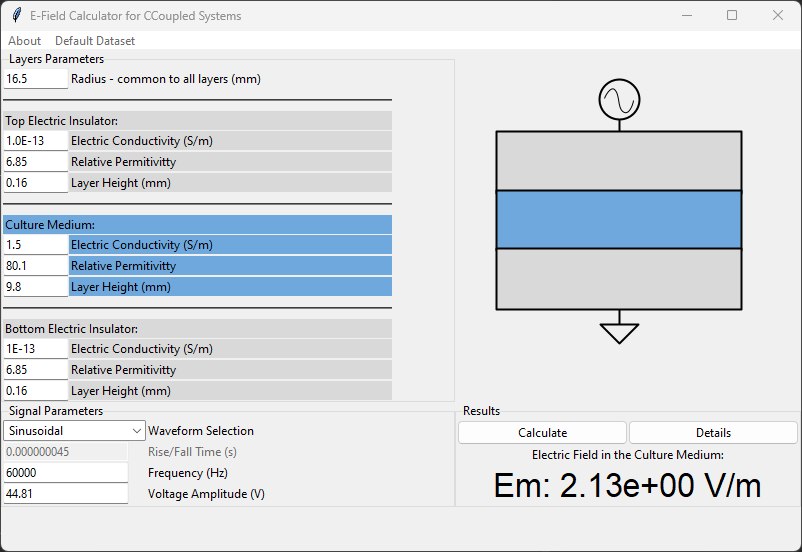
\includegraphics[scale=0.8]{./figures/Figure_5d11.png}}
\caption{Printscreen of the developed \acs{CCoupled} calculator graphical user interface displaying the magnitude of the \acs{EF} in the culture medium in the bottom right-hand corner for the setup reported in Brighton \textit{et al.}, 1992.}
\label{fig5d11}
\end{figure}  

Even though the laws of physics enable a reasonably accurate prediction of the \acs{EF} in the culture medium, the model should still be validated experimentally. Ideally, the \acs{EF} strength in the culture medium should be measured, but it may be difficult to do it correctly and accurately in most setups. Alternatively, the applied voltage and the current through the setup should be measured and reported. The ratio of these two quantities gives the total impedance of the setup, which can be compared with the value predicted by the model.

 

\section{Summary}

This chapter concluded that the effect of scaffold insertion on the \acs{EF} in the surrounding culture medium was mainly determined by the difference in electrical conductivity of these two materials (at low-frequency signals). The numerical simulations pointed to significant variations in local \acs{EF} patterns, which could lead to different cellular outcomes and confound the interpretation of the experimental results. According to the predictions, the presence of a scaffold can profoundly influence the \acs{EF} spatial patterns in its local environment by introducing local peaks and troughs or completely shielding the effects of external stimulation. The predicted \acs{EF} strongly depends on the electrical properties of the selected scaffold and culture medium. 

Also, this chapter showed a predominant overestimation of the \acs{EF} applied in reported \acs{CCoupled} stimulation studies. We analyzed eight CCoupled studies and sought to corroborate the reported estimates of the \acs{EF} in the culture medium. First, we reviewed the fundamental physics underlying \acs{CCoupled} stimulation and delineated three approaches to estimate the \acs{EF}. Using these approaches, we found that the reported values were overestimated in five studies, four based on incorrect assumptions. In all studies, insufficient information was provided to reproduce the setup exactly. Creating numerical models of experimental stimulation setups should improve the accuracy of the \acs{EF} estimates and enhance reproducibility. For this purpose, we developed a free, open-source tool, the \acs{EF} Calculator for \acs{CCoupled} systems, which is available for download from a public internet hosting platform.

At this point, the knowledge gathered in modelling different stimulation protocols, from mechanic stimulation due to fluid perfusion to \acs{EF} stimulation generated by \acs{DCoupled} or \acs{CCoupled} setups, was merged into the methodology of designing and constructing a singular bioreactor solution, which will be presented in the following chapter. 

%\newpage
%\bibliography{library_c5b} 
%\bibliographystyle{plain}
%\end{document}